% !TEX spellcheck = en_US
% !TEX encoding = UTF-8

\documentclass[a4paper, 12pt, dvipsnames]{book}

% !TEX root = main.tex

% Configuration file for the document

% \usepackage{scrextend} % KOMA-script
\usepackage{graphicx}
\usepackage[tuenc]{fontspec}
\usepackage{xcolor}
\usepackage{shellesc}

\usepackage{csquotes} % Required by biblatex
\usepackage[british]{babel}
\usepackage[
  backend=biber, 
  sorting=none, 
  dateabbrev=false, 
  block=ragged,
  style=ieee
]{biblatex}

\usepackage{tikz}
\usepackage{pgfgantt}
\usepackage{pgfplots}

\usepackage{amsmath, amsfonts, amssymb} % Font symbols
\usepackage{bm}

\usepackage[format=plain,
            labelfont={bf,it},
            textfont=it]{caption}
\usepackage{subcaption}
\usepackage{fancyvrb} % Verbatim improvements
\usepackage{fancyhdr}

\usepackage{float}
\usepackage{enumitem} % Continuous enumeration
\usepackage{ragged2e} % Justify

\usepackage{array} % Table improvements
\usepackage{multirow} % Multiple rows in tables
\usepackage{makecell} % Cell colors in tables
\usepackage{hhline}   % Better line separation in tables
\usepackage{tocloft}
\usepackage{lipsum}
\usepackage[nobottomtitles*]{titlesec}

%%%%%%%%% HYPERREF %%%%%%%%%%
\usepackage[colorlinks=true,
linkcolor={red!30!black},
citecolor={blue!50!black},
urlcolor={blue!80!black}]{hyperref}

% Must be loaded after hyperref
\usepackage[acronym, toc, numberline, nopostdot, xindy, style=index]{glossaries}
\usepackage[bindingoffset=1.5cm, textwidth=15cm, top=3cm, bottom=3cm]{geometry}


%%%%%%%% END OF INCLUDES %%%%%%%%%%

\pgfplotsset{compat=1.15}
\usetikzlibrary{positioning, external}
\tikzexternalize[
    optimize=false, 
    % mode=list and make
]
% \tikzset{%
%   % external/system call={lualatex \tikzexternalcheckshellescape --halt-on-error --interaction=batchmode --jobname "\image" "\texsource"},
%   external/system call={lualatex \tikzexternalcheckshellescape --halt-on-error --interaction=batchmode --output-directory=./build --jobname "\image" "\texsource"},
%   /pgf/images/include external/.code={%
%     \includegraphics{build/#1}%
%   },
% }

\setmainfont{CMU Serif}
\setmonofont[Scale=MatchLowercase]{Source Code Pro}
\setlength{\parskip}{\baselineskip}

\newcolumntype{P}[1]{>{\raggedright\arraybackslash}p{#1}}

% Bibliography
\addbibresource{../bibliography/mendeley.bib}

% Section defines
\newcommand{\secc}{\ifdef{\chapter}{\chapter}{\section}}
\newcommand{\ssecc}{\ifdef{\chapter}{\section}{\subsection}}
\newcommand{\sssecc}{\ifdef{\chapter}{\subsection}{\subsubsection}}

\newcommand{\seccn}{\ifdef{\chapter}{chapter}{section}}
\newcommand{\sseccn}{\ifdef{\chapter}{section}{subsection}}
\newcommand{\ssseccn}{\ifdef{\chapter}{subsection}{subsubsection}}
\newcommand{\Th}{\textsuperscript{th}}

\newcommand{\addphantomsec}[2]{%
  \cleardoublepage
  \phantomsection
  \addcontentsline{toc}{#2}{\numberline{}#1}
  \secc*{#1}
}

% Special heading, indenting the name on table of contents
\defbibheading{bibintocindent}[\refname]{%
  \secc*{#1}%
  \addcontentsline{toc}{\seccn}{\protect\numberline{}#1}%
  \markboth{\MakeUppercase{#1}}{\MakeUppercase{#1}}
}

\pagestyle{fancy}

\ifdef{\chapter}{
  \renewcommand\cftchapafterpnum{\vskip15pt}
  \renewcommand\cftsecafterpnum{\vskip6pt}
  \renewcommand\cftsubsecafterpnum{\vskip3pt}
  \renewcommand{\chaptermark}[1]%
             {\markboth{\thechapter\quad#1}{}}
  \renewcommand{\sectionmark}[1]%
              {\markright{\thesection\ #1}}
}{
  \renewcommand\cftsecafterpnum{\vskip15pt}
  \renewcommand\cftsubsecafterpnum{\vskip6pt}
}

\renewcommand\cftsubsubsecafterpnum{\vskip3pt}
\renewcommand\cftfigafterpnum{\vskip5pt}
\renewcommand\cfttabafterpnum{\vskip5pt}

% List configuration
\setlist[description]{topsep=0em}
\setlist[itemize]{topsep=0em, noitemsep}
\def\mscname{Joan Marcè i Igual}

\setlength{\headheight}{13.6pt} %add some space to headheight to eliminate LaTeX "Overfull \vbox..." warnings

\fancyhead[EL, OR]{\thepage}
\fancyhead[ER]{\rightmark}
\fancyhead[OL]{\MakeUppercase{\leftmark}}

\fancyfoot[C]{}
\fancyfoot[EL, OR]{\small\mscname}
\fancyfoot[ER, OL]{Bachelor Thesis}
\renewcommand{\footrulewidth}{0.4pt}



% !TEX root = main.tex

\makeglossaries

\newglossaryentry{test}{
  name=test,
  description={
    This is just a test
  }
}

\newglossaryentry{censoring}{
  name=censoring,
  description={
    If a subject does not have an event during the observation time, they are described as
    censored. This means that nothing is known about the subject after the censoring
  }
}

\newglossaryentry{baseline}{
  name={baseline data},
  symbol={\( \bm{x} \)},
  description={
    Available data to predict the survival time
  }
}

\newglossaryentry{time}{
  name=time,
  symbol={\( T \)},
  description={
    Time from the beginning of the observation period until an event, the end of the study
    or withdrawal from the study
  }
}

\newglossaryentry{event}{
  name=event,
  symbol={\( E \)},
  description={
    It can be death (\( E = 1 \)) or, otherwise, it can be recovery or withdrawal \( E = 0 \)
  }
}

\newglossaryentry{contrastive}{
  name={contrastive loss},
  description={
    Layer joining the two sister networks output to compare the distance between the outputs
  }
}

\newglossaryentry{leakage}{
  name={data leakage},
  description={
    Is a big problem in machine learning, happens when information from outside of the
    training set is used to create the model
  }
}

\newglossaryentry{train-pair}{
  name={train pair},
  description={
    Pair where the two members of the pair belong to the train set 
  }
}

\newglossaryentry{test-pair}{
  name={test pair},
  description={
    Pair where the two members of the pair belong to the test set
  }
}

\newglossaryentry{mixed-pair}{
  name={mixed pair},
  description={
    Pair where one member belongs to the test set and the other one to the train set
  }
}

\newglossaryentry{precision-medicine}{
  name={precision medicine},
  description={
    An emerging approach for disease treatment and prevention that takes into account individual 
    variability in genes, environment and lifestyle for each person
  }
}

\newacronym{UPC}{UPC}{Universitat Politècnica de Catalunya}
\newacronym{CFIS}{CFIS}{Centre de Formació Interdisciplinari Superior}
\newacronym{FIB}{FIB}{Facultat d'Informàtica de Barcelona}
\newacronym{CNN}{CNN}{Con\-vo\-lu\-tio\-nal Neural Networks}
\newacronym{MRI}{MRI}{Magnetic Resonance Imaging}
\newacronym{PET}{PET}{Positron Emission Tomography}
\newacronym{CT}{CT}{Computed Tomography}
\newacronym{CI}{CI}{Concordance Index}
\newacronym{ROC}{ROC}{Receiver Operating Characteristics}
\newacronym{OPSCC}{OPSCC}{Oropharyngeal Squamous Cell Carcinoma}
\newacronym{HNSCC}{HNSCC}{Head and Neck Squamous Cell Carcinoma}
\newacronym{CPH}{CPH}{Cox Proportional Hazards}
\newacronym{PMHNK}{PMHNK}{Princess Margaret Head and Neck}
\newacronym{DNN}{DNN}{Deep Neural Networks}
\newacronym{CC}{CC}{Compute Canada}
\newacronym{CV}{CV}{Cross Validation}
\newacronym{ML}{ML}{Machine Learning}
\newacronym{PNG}{PNG}{Portable Network Graphics}
\newacronym{UHN}{UHN}{University Health Network}
\newacronym{LOOCV}{LOOCV}{Leave One Out Cross Validation}
\newacronym{NN}{NN}{Neural Network}
\newacronym{GPU}{GPU}{Graphic Processor Unit}
\newacronym{CPU}{CPU}{Central Processor Unit}
\newacronym{PHI}{PHI}{Personal Health Information}
\newacronym{PHIPA}{PHIPA}{Personal Health Information Protection Act}
\newacronym{REB}{REB}{Research Ethics Board}
\newacronym{IP}{IP}{Intellectual Property}



%%%%%%%%%%%% BEGIN OF DOCUMENT %%%%%%%%%%%%%%%%%%
\begin{document}

% Title page can be commented to remove it
\begin{titlepage}
  \centering
  \vspace{1.5cm}
  {\huge \textbf{\textsc{Unlock the potential of medical imaging data using deep learning}} \par}
  \vspace{1cm}
  {\Large \textit{Joan Marcè i Igual}\par}
  \vfill
  {Director: Dr.~Benjamin \textsc{Haibe-Kains} \par}
  {Tutor: Dr.~Maria José \textsc{Serna Iglesias} \par}
    
  \vfill

  
\includegraphics[width=0.3\textwidth]{images/logo_FIB}\par
  
  \vspace{.2cm}
  
  
\includegraphics[width=0.6\textwidth]{images/logo_upc}\par
  
  \vfill
  
  % Bottom of the page
  {\Large Computer Science Specialization \par}
  {\LARGE Facultat d'Informàtica de Barcelona \par}
  {\LARGE Universitat Politècnica de Catalunya \par}
  {\LARGE 2018 \par}
\end{titlepage}

\thispagestyle{empty}

\cleardoublepage
\pagenumbering{roman}
% !TEX root = ../main.tex

\secc*{Abstract}
\markboth{ABSTRACT}{ABSTRACT}

\lipsum[3]

\cleardoublepage
\pagenumbering{arabic}
\tableofcontents

\cleardoublepage
\phantomsection
\addcontentsline{toc}{\seccn}{\numberline{}List of Figures}
\listoffigures

\cleardoublepage
\phantomsection
\addcontentsline{toc}{\seccn}{\numberline{}List of Tables}
\listoftables

% Just comment this lines to enable/disable some parts of the document
\cleardoublepage
% !TEX root = ../main.tex

\secc[Context]{Context and scope of the project}
\ssecc{Context}

Nowadays one of the most extensive uses of computing is artificial intelligence. A few 
examples are Amazon purchase recommendations, based on previous purchases, or help users
to interact with their phone by only using voice commands like Google Assistant 
~\cite{neural:amazon, neural:google-assistant}.

Inside AI one of the domains that has greatly increased during the last years is 
\gls{ML}. The main advantage is that it can solely learn from examples without explicit 
teaching, and thus reducing the human interaction during the learning process. One of the 
most used types is \emph{deep neural networks} and these have demonstrated impressive 
performance against computer vision and Natural Language Processing tasks like the 
classification of digits from the MNIST data set
~\cite{neural:mnist, neural:empirical-evaluation-deep-architectures}.

Regarding the medical field, recent deep learning algorithms, specially \gls{CNN} 
have started to push the boundaries of precision medicine. Traditionally, medical 
predictions have been based on a few clinical parameters with poor accuracy.
However, other data types are available to improve such predictions. In this context, 
medical images generated from \gls{MRI}, \gls{PET} or \gls{CT} scans are vastly 
underused due to the inability of radiologists to quantitatively analyze these 
complex data.

Different methods have appeared to analyze these images for tasks such as image 
classification, object detection, segmentation and registration among other tasks. This
approach started in the late 1990s and has slowly shifted from systems that are 
completely designed by humans to systems that are trained by computers using example data
~\cite{medical:survey-deep-learning}.

Professor Benjamin Haibe-Kains has participated in one of the seminal studies in 
\emph{Radiomics} (Nat Comm). \emph{Radiomics} is a new field, relying on pre-defined, 
hand-engineered features computed from medical images, to better characterize tumours 
and predict survival outcome.

High-dose radiotherapy with or without chemotherapy is the standard of care for many
locally advanced cancers, \emph{oropharynx cancer}. While effective in some patients,
these treatments are associated with significant risks of early and late toxicities
that impair patients' treatment adherence and long-term quality of life. Furthermore, 
most cancers are currently treated with a one-size-fits-all approach that invariably leads
to over-treatment of som patient and under-treatment of others. 
The clinical implication of this is that some patients are cured by the standard 
one-size-fits-all treatments currently employed while others are not 
~\cite{medical:personalized}. Refined prognostic 
models are needed to assist clinicians in delivering the appropriate level of care.

Radiomics is an emerging field of research that can non-invasively quantify tumour 
phenotypes, based on mining and extracting a large number of quantitative imaging 
features ~\cite{medical:radiomics:data, medical:radiomics:extract-information}.
It is aimed at using computational techniques to extract
the most informative features from radiological images routinely used in clinical settings.
Recent studies have demonstrated the effectiveness of radiomic features as biomarkers 
associated with survival of patients with lung and head and neck cancers. Conventional
radiomic pipelines comprise four main components:
\begin{itemize}
  \item Image acquisition
  \item Extracting hand-engineered features
  \item Assessing their robustness
  \item Building predictive models based on the most relevant features
\end{itemize}

Different machine learning approaches, such as \glspl{NN}, have been applied for the last 
step of the pipeline. However, recent advances have allowed for more complex (deeper) 
\glspl{NN}, and have led to unique feature learning properties with unprecedented performance
for image classification. Contrary to the conventional radiomic models, deep networks
eliminate the need for hand-engineered features, which may not necessarily be the most
relevant set of features for prognostication of cancer patients.

Although promising, radiomics suffers from several 
limitations. The most important one is that it relies on hand-engineered features, 
these features are not guaranteed to be the most discriminant ones. Deep learning methods
are end-to-end and, for a given task, they drive features from the data
~\cite{medical:radiomics-ml-classifiers}.

\sssecc{Survival Analysis}
\label{sec:survival}

Survival Analysis is a branch of statistics that analyzes the duration time of the observed
events. Typically it refers to the time to the failure of a physical component or to death of a
patient. It usually defines the following terms~\cite{neural:survival-analysis}:

\begin{description}
  \item[\Gls{event} \glssymbol{event}] \glsdesc*{event}
  \item[\Gls{time} \glssymbol{time}] \glsdesc*{time}
  \item[\Gls{baseline} \glssymbol{baseline}] \glsdesc*{baseline}
  \item[\Gls{censoring}] \glsdesc*{censoring}
\end{description}

The survival and hazard functions are the two fundamental functions in survival analysis. The
survival function \( S(t) = \Pr(T \ge t) \), is the probability that an individual has
\emph{survived} beyond time \( t \). The hazard function \( \lambda(t) \) is a measure of risk at 
time \( t \) and it's defined as:
~\cite{medical:cox}
\[
  \lambda(t) = \lim_{\Delta t \rightarrow 0}
  \frac{\Pr(t \le T < t + \Delta t | T \ge t)}{\Delta t}
\]

Usually, when trying to fit a survival model a \gls{CPH} model is used. This type of model
intends to use the \gls{baseline} \( \bm{x} = (x_1, x_2, ..., x_p) \)
to fit the hazard function \( \lambda(t) \)
in the following way:
\[
  \lambda(t | \bm{x}) = \exp(\bm{x}\bm{\beta}) \cdot \lambda_0 (t)
\]
Where \( \bm{\beta} \) is a \( p \times 1 \) vector of unknown parameters, that need to be fit, 
and \( \lambda_0(t) \) is an unknown function giving the standard set of conditions 
\( \bm{x} = \bm{0} \). As it can be seen this model requires for a log-linear relation between
the \gls{baseline} \glssymbol{baseline} and the hazard function \( \lambda(t | \bm{x}) \).

However, casting the survival analysis as a ranking problem is a way of dealing with the biased
distributions of survival times and the censoring data. Two subjects' survival times can be 
ordered only if:
\begin{itemize}
  \item Both of them are uncensored (\( \bm{E}_i = \bm{E}_j = 1\))
  \item The uncensored time of one is smaller than the censored survival time of the other
  (\( \bm{T}_i < \bm{T}_j | \bm{E}_i = 1; \bm{E}_j = 0 \))
\end{itemize}

This can be visualized by means of an order graph \( G = (V, E) \), see \autoref{fig:graph-ci}.
The set of vertices \( V \) represents all the individuals, where each filled circle 
(\( \bullet \)) indicates an \emph{uncensored} survival time, while an empty circle 
(\( \circ \)) denotes a \emph{censored} observation.
Existence of an edge \( E_{ij} \) implies that \( \bm{T}_i < \bm{T}_j \). An edge cannot originate 
from a censored point.

\begin{figure}
  \centering
  \begin{subfigure}[b]{.4\textwidth}
    \centering
    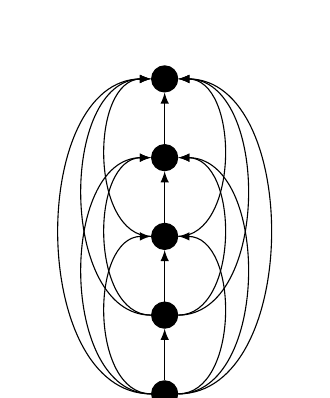
\begin{tikzpicture}
  \tikzstyle{bDot}=[circle, fill=black, draw]
  \foreach \y in {1,...,5} {
    \node[bDot] (D-\y) at (0, \y) {};
  }

  \foreach \y in {1,...,4} {
    \pgfmathsetmacro{\z}{int(\y + 1)}
    \draw[-latex] (D-\y) -- ({D-\z}.south);
  }

  \foreach \y in {1,...,3} {
    \pgfmathsetmacro{\z}{int(\y + 2)}
    \foreach \j in {\z,...,5} {
      \ifthenelse{\y=2 \OR \y=3}{
        \draw[-latex] (D-\y) to[bend left=90] (D-\j);
      }{
        \draw[-latex] (D-\y) to[bend right=90] (D-\j);
      }
    }
  }
\end{tikzpicture}

    \caption{Without censored data}
  \end{subfigure}
  ~
  \begin{subfigure}[b]{.4\textwidth}
    \centering
    \begin{tikzpicture}
  \foreach \y in {1,...,5} {
    \ifthenelse{\y=2 \OR \y=4}{
      \node [circle, fill=white, draw=black] (D-\y) at (0, \y) {};
    }{
      \node [circle, fill=black, draw=black] (D-\y) at (0, \y) {};
    }

    \foreach \y in {3,4,5} {
      \draw [-latex] (D-1) to[bend right=90] (D-\y);
    }

    \foreach \y/\z in {1/2, 3/4} {
      \draw [-latex] (D-\y) -- (D-\z);
    }
    \draw [-latex] (D-3) to[bend left=90] (D-5);
  }
\end{tikzpicture}

    \caption{With censored data}
    \label{fig:graph-ci:censored}
  \end{subfigure}

  \caption[Order graph with ranking constraints]{
    Order graphs representing the ranking constraints \label{fig:graph-ci}
    
    Censored data is represented by \( \circ \) and uncensored data is represented by \( \bullet \).
    Every edge \( A \rightarrow B \) means \( T_A > T_B \). Note that in 
    \autoref{fig:graph-ci:censored} some vertex are not connected since an edge 
    \( \circ \rightarrow \bullet \) cannot be formed.
  }
\end{figure}

% C-index explanation
The standard performance measure, to compare if a survival 
model is performing better than another, is the \gls{CI}. To obtain this 
indicator, pairs are generated to compare the survival time. A prediction is counted as good only
if both \( T_i > T_j \) and \( \hat{T}_i > \hat{T}_j \), otherwise
it's counted as a bad prediction, note that \( T_i = \hat{T}_i \) it's not a required condition. 
Then, the number of good predictions is divided by the total predictions. 
~\cite{medical:ranking-ci}

\[
  CI = \frac{\text{Good predictions}}{\text{Total predictions}} \in [0, 1]
\]

Also, another comparison 
element is the \gls{ROC} curve which represents the \emph{False Positive Rate} against the 
\emph{True Positive Rate}, see \autoref{fig:ROC-curve}. Usually the \gls{CI} is seen as 
the area under the \gls{ROC} curve.
~\cite{neural:roc-precision-recall}

\begin{figure}
  \centering
  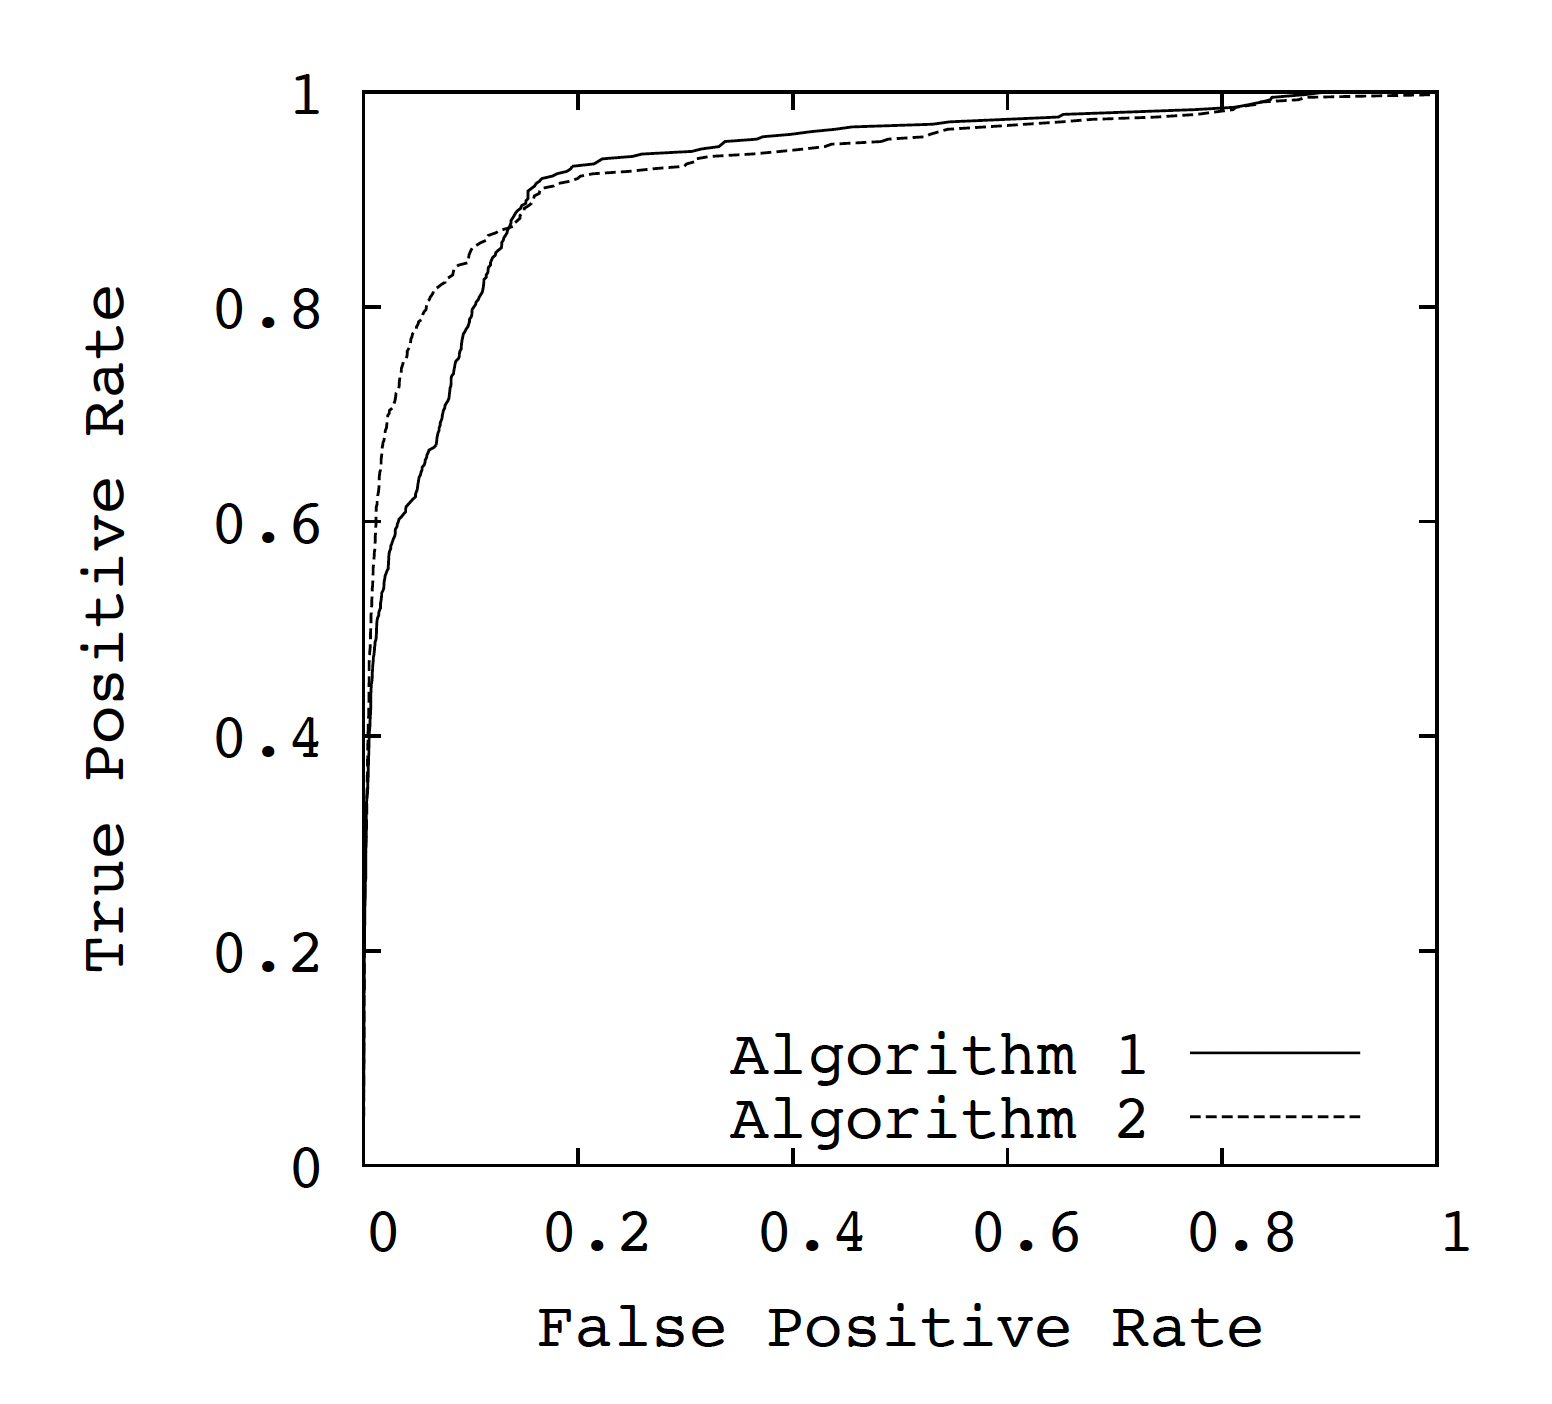
\includegraphics[width=.5\linewidth]{images/roc_curve}
  \caption{\acrshort{ROC} Curve example\label{fig:ROC-curve}}
\end{figure}

\sssecc{Dataset}

The dataset used by this project to develop a model is provided through a 
collaboration with Dr.~Fei-Fei Liu, head of the Radiation Medicine Program at Princess
Margaret Cancer Centre.

We have access to a unique set of 671 cancer patients diagnosed of \gls{OPSCC}. Accounting
for approximately half a million cases annually worldwide, \gls{HNSCC} 
is a considerable cause of mortality and morbidity, with the majority of patients having
locally advanced, unresectable disease. \gls{OPSCC} has been one of the fastest growing 
disease sites for \gls{HNSCC}.
~\cite{medical:ct-based-radiomic-signature}

Multiple information is provided for each patient. There's a \gls{CT} scan, where the tumour 
can be seen, and clinical information about the patient. The scan is 512 pixels wide by 512 
pixels tall and is composed of 100-200 slices in gray scale that together form a 3D image. 
To be able to slice the tumour from the rest of the image, a mask of the same size as the scan 
is provided. The masks contains information about the tumour location, it has \texttt{1}s 
in the pixels containing the tumour and \texttt{0}s
otherwise, as it can be seen in \autoref{fig:dataset-example}.

In the following document we will be calling this the \gls{PMHNK} dataset.

Regarding the clinical information the following fields are provided:
\begin{itemize}
  \item Subject characteristics (age, gender, clinical status, smoking, drinking history)
  \item Tumor characteristics (cancer location, staging, p16 status)
  \item Treatment data (modality, radiation start/end dates, radiation dose/fractionation, 
  treatment completion status)
  \item Outcome data (status, cause of death, local failure, regional failure, distant failure)
\end{itemize}

\begin{figure}
  \centering
  \begin{subfigure}[t]{.32\textwidth}
    \centering
    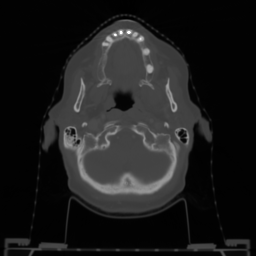
\includegraphics[width=\textwidth]{images/IMG0138_example.png}
    \caption{Original image}
  \end{subfigure}
  \hfill
  \begin{subfigure}[t]{.32\textwidth}
    \centering
    
\includegraphics[width=\textwidth]{images/IMG0138_MASS_example.png}
    \caption{Image mask}
  \end{subfigure}
  \hfill
  \begin{subfigure}[t]{.32\textwidth}
    \centering
    
\includegraphics[width=\textwidth]{images/IMG0138_merge_example.png}
    \caption{Mask applied to original}
  \end{subfigure}

  \caption[Images from the dataset]{
    Example of images from the dataset \label{fig:dataset-example}
    
    Single \gls{CT}'s scan slice, a whole scan is composed of multiple slices. By applying 
    the mask to the original image, the part that only contains the tumour can be extracted.
  }
\end{figure}


\sssecc{Neural Networks}

Neural Networks are a class of \gls{ML} algorithms. The idea is to extract multiple 
linear combinations of the inputs as derived features and model the objective as a nonlinear
function of these features. As it has been previously explained this is a powerful learning
method which has had really good results in many fields.
~\cite{neural:elements-statistical-learning}

A neural network is a two-stage regression or classification algorithm, typically represented
by a graph (or network) diagram as seen in \autoref{fig:neural_network}. It is composed by 
\( L \) layers and each layer has multiple units. The number of units in layer \( l \) 
is defined by  \( n^{[l]} \).

Each hidden unit has an activation (output) computed in two steps, the linear and the 
non-linear step, these are represented by \( \bm{z} \) and \( \bm{a} \) respectively.
These are called hidden units because the values of \( \bm{z} \) and \( \bm{a} \) are 
not directly observed. In general, more than one hidden unit is used to fit more complex 
features.

The linear step is performed by adding each output from the
previous layer (\( l - 1 \)), multiplying it by a weight and adding a bias.
Here, \(w_{ij}^{[l]}\) denotes a weight between unit \( j \) of layer \( l - 1 \) 
and unit \( i \) of layer \( l \). 

The non-linear step is defined by applying a non-linear function, called activation, 
(\( g^{[l]} \)) to the linear part. 
Multiple activation functions can be seen in \autoref{fig:activation_functions}. Depending
on the application, a different activation function may be used, for example in 
\glspl{CNN} usually the ReLU function is used due to the low computational complexity. 
These are defined as:
~\cite{neural:bishop}
\begin{itemize}[itemsep=1ex]
  \item Rectified Linear Unit function 
  \( g(x) = \max(0, x) \)
  \item Hyperbolic tangent function 
  \( \displaystyle g(x) = \tanh(x) = \frac{e^x - e^{-x}}{e^x + e^{-x}}\)
  \item Logistic function 
  \( \displaystyle g(x) = \frac{1}{1 + e^{-x}} \)
\end{itemize}

So, the whole activation for unit \( i \) of layer \( l \) is as follows:
\begin{align*}
  z_i^{[l]} &= \sum_{j = 1}^{n^{[l]}} w_{ij}^{[l]} + w_{i0}^{[l]} \cdot a_j^{[l - 1]} \\
  a_i^{[l]} &= g^{[l]}(z_i^{[l]})
\end{align*}

By using a matrix notation, it can be applied to the whole layer's units:
\begin{align*}
  \bm{z}^{[l]} &= \bm{W}^{[l]} \cdot \bm{a}^{[l - 1]} + \bm{b}^{[l]} \\
  \bm{a}^{[l]} &= g^{[l]}(\bm{z}^{[l]})
\end{align*}


\begin{figure}
  \centering
  \tikzset{
  pics/layer/.style n args = {3}{
    code = {
      \ifthenelse{\equal{#3}{H}}{
        \def\cellcolor{red!20}
      }{
        \ifthenelse{\equal{#3}{I}}{
          \def\cellcolor{green!20}
        }{
          \def\cellcolor{Cyan!20}
        }
      }

      \foreach \y in {1,...,#1} {
        \node[draw, circle, fill=\cellcolor] 
          (L-#2-\y) at (0,{1.5*(#1/2 - \y)}) {${#3}_{\y}^{[#2]}$};
      }
    }
  }
}

\begin{tikzpicture}

\def\layers{2/I, 4/H, 4/H, 3/O}

\foreach \x/\name [count=\xi] in \layers  {
  \draw (3*\xi, 0) pic {layer={\x}{\xi}{\name}};
}

\foreach \x/\ignore [count=\xi, remember=\xi as \lastxi, remember=\x as \lastx] in \layers {
  \ifthenelse{\xi > 1}{
    \foreach \ylast in {1,...,\lastx} \foreach \y in {1,...,\x}{
      \draw [-latex] (L-\lastxi-\ylast) -- (L-\xi-\y);
    }
  }{};
}

\draw (L-1-1) -- (L-2-1) node[midway, sloped, above] {\( w_{ij} \)};

\end{tikzpicture}


  \caption[Neural network graph]{
    Neural Network graph drawing. 
    \label{fig:neural_network}
    
    Each circle represents a unit, green means input, red hidden and blue a output unit.
    In this case the network has 2 units for the input layer, 2 hidden layers with 4 units
    each and 3 units in the output layer.

    Each arrow represents a weight $w_{ij}^{[l]}$ between two units.
  }
\end{figure}
\begin{figure}
  \centering
  
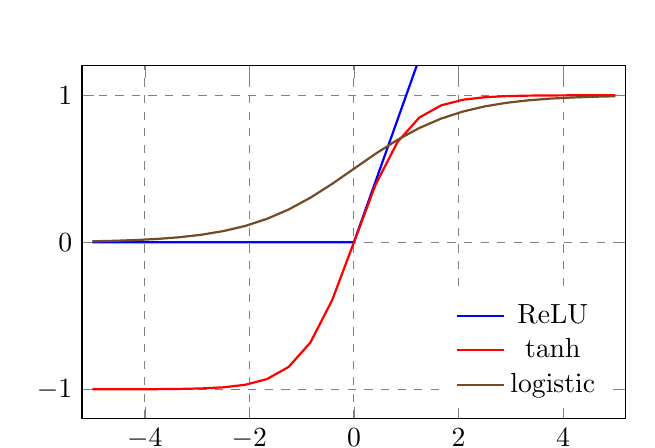
\begin{tikzpicture}
\begin{axis}[
    xmin = -5.2, xmax = 5.2,
    ymin = -1.2, ymax = 1.2,
    legend style = {draw = none},
    legend pos = south east,
    grid=major,
    grid style = {dashed, gray},
    width = 0.7\textwidth,
    height = 0.5\textwidth,
    every axis plot/.append style={thick},
    no markers,
    cycle list name = color
  ]
  \addplot{max(0, x)};
  \addplot{tanh(x)};
  \addplot{1/(1 + exp(-x))};
  \legend{ReLU, tanh, logistic}
\end{axis}
\end{tikzpicture}

  \caption[Activation functions]{
    Activation functions.
    \label{fig:activation_functions}
  }
\end{figure}

The output units allow for a final transformation of the previous layer's vector of outputs.
For regression, typically the identity function \( g^{[L]}(\bm{a^{[L - 1]}}) = \bm{a^{[L - 1]}} \)
is chosen. However, if \( K \)-class classification is going to be used usually the
\emph{softmax} function is used instead. This function provides a probability for each
one of the \( K \) classes:
\[
  g_k^{[L]}(\bm{a}^{[L - 1]}) = \frac{e^{a_k^{[L - 1]}}}{\sum_{i = 1}^K e^{a_i^{[L - 1]}}}
\]

As it has been said, a \gls{NN} has unknown parameters \( \bm{W}^{[l]} \), called weights, and the objective is
to find the values that make the model fit the training data well. The cost function 
is the objective function to be minimized, for regression it's usually defined as 
the mean squared error:

\begin{align*}
  \hat{\bm{y}} &:= g^{[L]}(\bm{a^{[L - 1]}}) \\
  C(\bm{y}, \hat{\bm{y}}) &:= \frac{1}{N} \sum_{i = 1}^N (y_i - \hat{y}_i)^2
\end{align*}

To minimize the objective function, the gradient descent algorithm is used. It is an iterative
algorithm that updates the weights by partial derivative of the cost function with respect to 
the weight. The amount to be updated is defined by the learning rate \( \alpha \):
\begin{align*}
  \underbrace{w_{ij}^{[l]}}_{\text{new}} = \underbrace{w_{ij}^{[l]}}_{\text{old}} - \alpha 
  \frac{\partial C(\bm{y}, \hat{\bm{y}})}{\partial w_{ij}^{[l]}}
\end{align*}

To update all the network's parameters the back-propagation algorithm is used. It's based
in the chain rule derivative and it updates the parameters from the last layer to the first
one.
~\cite{neural:efficient-backprop}


\sssecc{Convolutional Neural Networks}

\glspl{CNN} are a subset of \glspl{NN}. These networks are used for tasks such as 
computer vision due to the high accuracy that can be achieved in image recognition problems.
They can be accelerated through hardware such as \glspl{GPU}. Even though they can be used 
without \glspl{GPU} the operations can be really optimized by these type of processors. 

The convolution operator is denoted by \( * \). In \gls{ML}, the input is usually 
a multi-dimensional array and the convolution kernel is usually another multi-dimensional
array of parameters that are learned by the learning algorithm. When working with 
convolutions, the kernel matrix is flipped before performing the operations. However,
many \gls{NN} libraries perform the cross-correlation operation, which is the same
but without flipping the kernel. A graphical example of the convolutional operation 
can be seen in \autoref{fig:conv-operation}.
~\cite{neural:deeplearning-book}

Usually, a convolutional layer is defined by four parameters:
\begin{description}[topsep=0em]
  \item[Padding] \( p \) amount of extra space added around the matrix being convoluted, 
  usually in form of 0s. This defines the following terms:
  \begin{description}
    \item[Same] Add padding so the output size ends up being the same as the input size
    \item[Valid] Do not add padding at all
  \end{description}
  \item[Stride] \( s \) displacement of the filter
  \item[Filter size] \( f \) size of the filter matrix, usually it has the same width as height but
  it's not mandatory.
  \item[Number of filters] amount of different kernels that will be used to filter the input
  image to generate multiple images as output. It can be seen as filtering first the 
  vertical lines, then the horizontal ones and so on.
\end{description}

Having all the parameters, if one of the dimension's input size is \( n_{\text{prev}} \)
the output size will be defined by:
\begin{align*}
  n_{\text{next}} = \left\lfloor\frac{n_{\text{prev}} + p - f}{s}\right\rfloor + 1
\end{align*}

\begin{figure}
  \centering
  
\usetikzlibrary{matrix, positioning}
\begin{tikzpicture}
  \matrix (mtr) [matrix of nodes,row sep=-\pgflinewidth, nodes={draw}]
	{
		0 & 1 & 1 & |[fill=red!30]| 1 & |[fill=red!30]| 0 & |[fill=red!30]| 0 & 0\\
		0 & 0 & 1 & |[fill=red!30]| 1 & |[fill=red!30]| 1 & |[fill=red!30]| 0 & 0\\
		0 & 0 & 0 & |[fill=red!30]| 1 & |[fill=red!30]| 1 & |[fill=red!30]| 1 & 0\\
		0 & 0 & 0 & 1 & 1 & 0 & 0\\
		0 & 0 & 1 & 1 & 0 & 0 & 0\\
		0 & 1 & 1 & 0 & 0 & 0 & 0\\
		1 & 1 & 0 & 0 & 0 & 0 & 0\\
  };
  
  \draw[very thick, red] (mtr-1-4.north west) rectangle (mtr-3-6.south east);

	\node [below= of mtr-5-4.south] (lm) {$\bf I$};

	\node[right = 0.2em of mtr] (str) {$*$};

	\matrix (K) [right=0.2em of str,matrix of nodes,row sep=-\pgflinewidth, nodes={draw, fill=blue!30}]
	{
		1 & 0 & 1 \\
		0 & 1 & 0 \\
		1 & 0 & 1 \\
	};
	\node [below = of K-3-2.south] (lk) {$\bf K$};

	\node [right = 0.2em of K] (eq) {$=$};

	\matrix (ret) [right=0.2em of eq,matrix of nodes,row sep=-\pgflinewidth, nodes={draw}] {
		1 & 4 & 3 & |[fill=green!30]| 4 & 1\\
		1 & 2 & 4 & 3 & 3\\
		1 & 2 & 3 & 4 & 1\\
		1 & 3 & 3 & 1 & 1\\
		3 & 3 & 1 & 1 & 0\\
	};
	\node [below = of ret-4-3.south] (lim) {${\bf I} * {\bf K}$};

	\draw[very thick, green] (ret-1-4.north west) rectangle (ret-1-4.south east);

	\draw[densely dotted, blue, thick] (mtr-1-4.north west) -- (K-1-1.north west);
	\draw[densely dotted, blue, thick] (mtr-3-4.south west) -- (K-3-1.south west);
	\draw[densely dotted, blue, thick] (mtr-1-6.north east) -- (K-1-3.north east);
	\draw[densely dotted, blue, thick] (mtr-3-6.south east) -- (K-3-3.south east);

	\draw[densely dotted, green, thick] (ret-1-4.north west) -- (K-1-1.north west);
	\draw[densely dotted, green, thick] (ret-1-4.south west) -- (K-3-1.south west);
	\draw[densely dotted, green, thick] (ret-1-4.north east) -- (K-1-3.north east);
	\draw[densely dotted, green, thick] (ret-1-4.south east) -- (K-3-3.south east);

	\matrix (K) [right=0.2em of str,matrix of nodes,row sep=-\pgflinewidth, nodes={draw, fill=blue!10}] {
		1 & 0 & 1 \\
		0 & 1 & 0 \\
		1 & 0 & 1 \\
	};

	\draw[very thick, blue] (K-1-1.north west) rectangle (K-3-3.south east);

	\node[anchor=south east, inner sep=0.01em, blue] at (mtr-1-4.south east) (xx) {\scalebox{.5}{$\times 1$}};
	\node[anchor=south east, inner sep=0.01em, blue] at (mtr-1-5.south east) (xx) {\scalebox{.5}{$\times 0$}};
	\node[anchor=south east, inner sep=0.01em, blue] at (mtr-1-6.south east) (xx) {\scalebox{.5}{$\times 1$}};
	\node[anchor=south east, inner sep=0.01em, blue] at (mtr-2-4.south east) (xx) {\scalebox{.5}{$\times 0$}};
	\node[anchor=south east, inner sep=0.01em, blue] at (mtr-2-5.south east) (xx) {\scalebox{.5}{$\times 1$}};
	\node[anchor=south east, inner sep=0.01em, blue] at (mtr-2-6.south east) (xx) {\scalebox{.5}{$\times 0$}};
	\node[anchor=south east, inner sep=0.01em, blue] at (mtr-3-4.south east) (xx) {\scalebox{.5}{$\times 1$}};
	\node[anchor=south east, inner sep=0.01em, blue] at (mtr-3-5.south east) (xx) {\scalebox{.5}{$\times 0$}};
  \node[anchor=south east, inner sep=0.01em, blue] at (mtr-3-6.south east) (xx) {\scalebox{.5}{$\times 1$}};
  
  \node [right = .5 of ret] {\(
    \begin{aligned}
      &1 \cdot 1 + 0 \cdot 0 + 0 \cdot 1\ + \\
      &1 \cdot 0 + 1 \cdot 1 + 0 \cdot 0\ + \\
      &≈1 \cdot 1 + 1 \cdot 0 + 1 \cdot 1 = 4
    \end{aligned}
  \)};
\end{tikzpicture}


  \caption[Convolution operation example]{
    Example of Convolution operation applied to a \( 5 \times 5 \) matrix with a 
    \( 3 \times 3 \) filter and with padding \( p = 1 \) added to the input matrix. 
    The output is a \( 5 \times 5 \) matrix.
    \label{fig:conv-operation}
  }
\end{figure}

To form the convolutional layer, the matrix multiplication with the previous layer's 
activation vector gets replaced by the convolution operation over the activation 
matrix. 
\begin{align*}
  \bm{z}^{[l]} &= \bm{W}^{[l]} \cdot \bm{a}^{[l - 1]} + \bm{b}^{[l - 1]} \\
  &\downarrow \text{becomes} \\
  \bm{\mathsf{Z}}^{[l]} &= \bm{\mathsf{A}}^{[l - 1]} * \bm{\mathsf{W}}^{[l]} + 
  \bm{\mathsf{B}}^{[l - 1]}
\end{align*}

\ssecc{State-of-the-art}

Nowadays, a lot of research is being done in the medical field using deep learning. Image
classification is one of the first areas in which there's a major contribution to medical analysis.
Usually in image classification there are one or multiple images as input and a single diagnostic 
variable as output (e.g.~ill or not).
~\cite{medical:survey-deep-learning}

Regarding the prediction of survival models, there have been different approaches although
almost all of them use \gls{MRI}, \gls{PET} or \gls{CT} scans and the clinical data. 
The typical one, is to extract hand-crafted radiomic features using own methods or using 
libraries such as \emph{PyRadiomics}. This 
hand-crafted features are usually based in aspects like tumour shape, intensity, volume or texture.
~\cite{medical:tumour-radiomics, medical:py-radiomics, medical:computational-radiomics}

An alternative approach, is to use a deep learning-based model for prediction and for feature
extraction. In this case, features are extracted too but a \gls{CNN} 
is used instead. With this approach, the use of transfer learning has been a
great improvement. Also, pre-trained networks are used to reduce the requirement of large data
sets for deep network training. Usually, there are two possible strategies: 
\begin{itemize}
  \item Using a pre-trained NN as a feature extractor
  \item Fine-tuning a pre-trained network on medical data.
\end{itemize}

Both strategies are popular and have been widely applied. A network that allows this type
of retrain is GoogLeNet Inception v3
~\cite{neural:goog-le-net, neural:retrain, neural:inception-retrain}.
However, there's the added problem that medical imaging data are usually 3D images but, 
when working with pre-trained \gls{CNN}, only 2D images can be used, because there are still no 
pre-trained networks on 3D images. Although this method seems promising, still requires 
further work to train a dedicated feature extractor explicitly designed for medical images.
~\cite{medical:deep-learning-radiomics-gbm}

An implemented survival prediction model is \emph{DeepSurv} which is based on survival data
and uses the \gls{CPH} model for an individual's survival given the \gls{baseline}
\( x \). It's an Open Source Python module that applies recent deep learning techniques 
to a Cox model.
~\cite{medical:deep-surv, medical:cox}

In the 3D imaging field, there has been some work too. 3D \glspl{CNN} have
been used for brain lesion segmentation on multi-channel \gls{MRI} scans. In this case a 
dual pathway of 11-layers deep 3D \gls{CNN} was used and was able to improve the previous
state-of-the art, the model structure can be seen in \autoref{fig:deepmedic} and the code 
can be found on GitHub. 
One of the biggest handicaps found was the computational intensity of
processing 3D medical scans, since they usually need a lot of memory and GPU time.
~\cite{neural:deepmedic, neural:3d-cnn-crf}

\begin{figure}
  \centering
  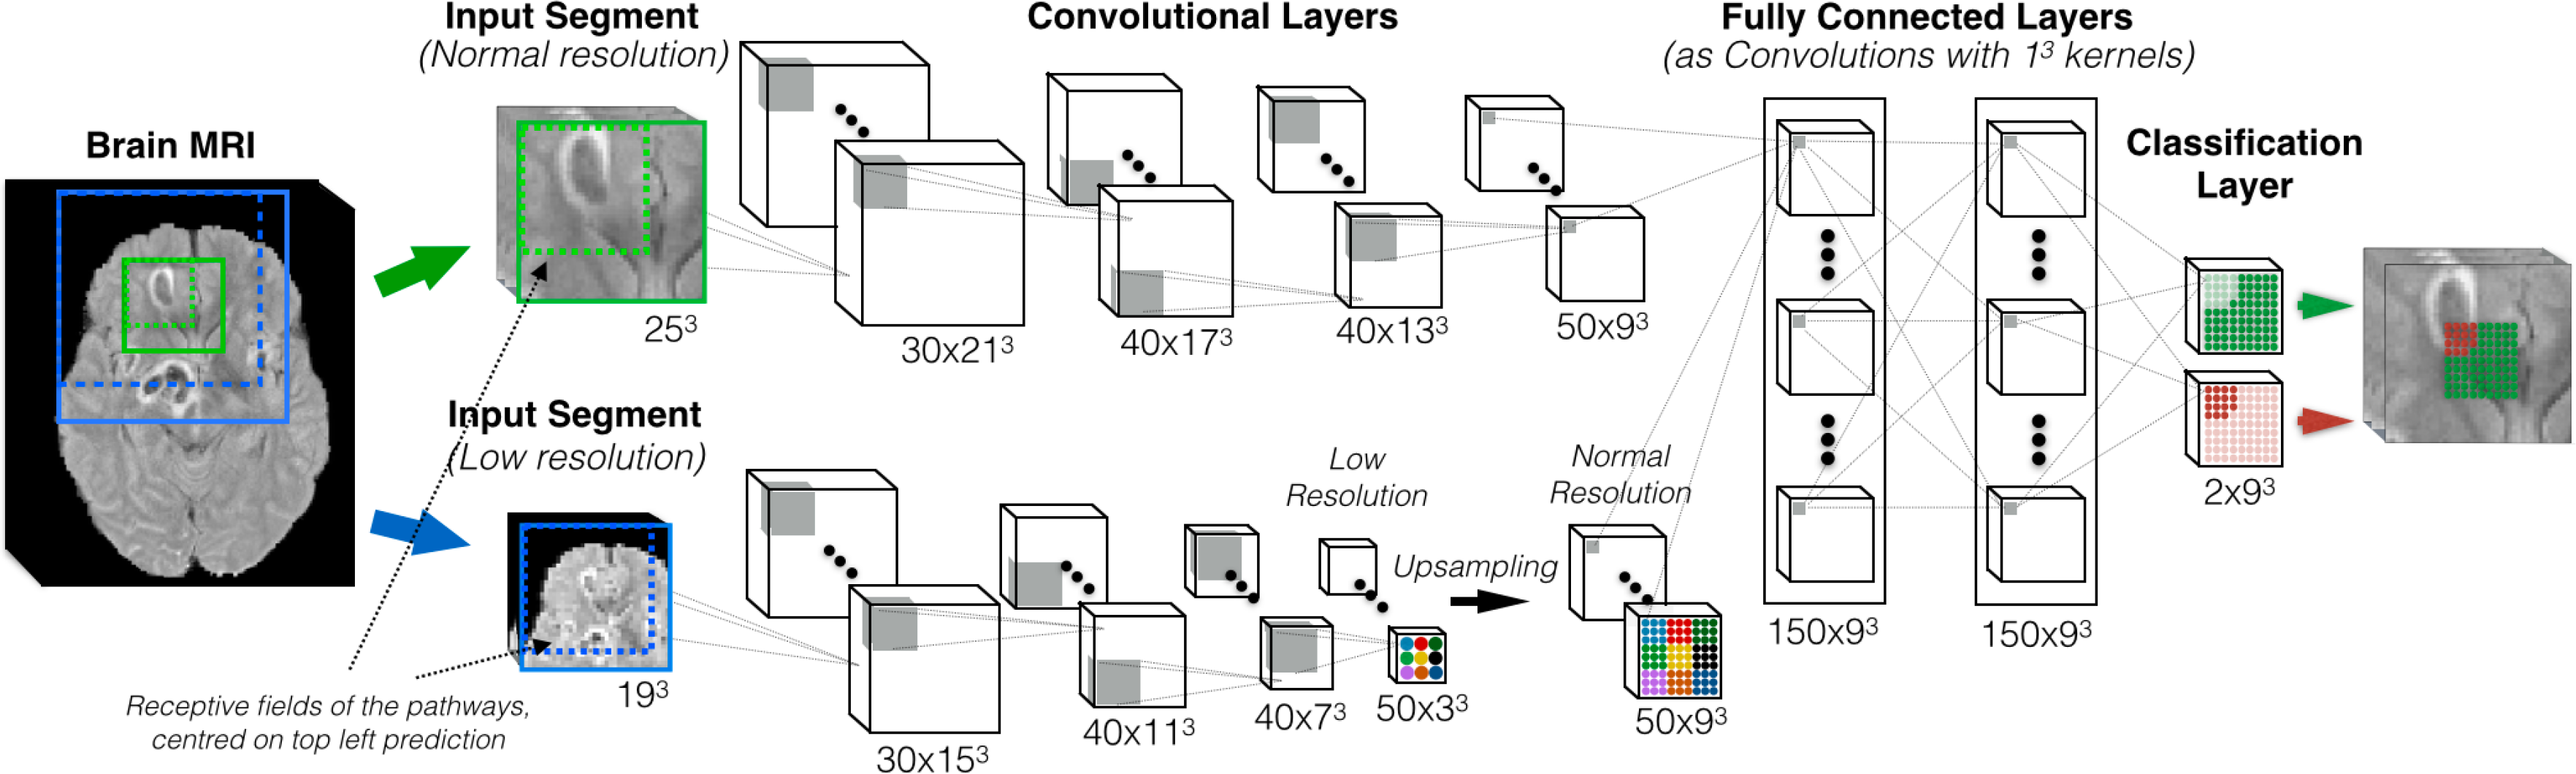
\includegraphics[width=\textwidth]{images/deepmedic}

  \caption[DeepMedic 3D CNN model]{
    DeepMedic 3D \acrshort{CNN} model for brain lesion segmentation \cite{neural:3d-cnn-crf}
    \label{fig:deepmedic}
  }
\end{figure}

Another application of 3D \glspl{CNN} has been in action detection and segmentation for videos.
In this case video imaging was treated as a 3D image where the 3rd dimension represents
time.
~\cite{neural:3d-cnn-action-detection}

On the \gls{PMHNK} dataset some results have already been obtained. By using the \gls{CT} scans and
extracting some features. In this case, the extracted features were:
\begin{itemize}
  \item First order statistics: Energy
  \item Shape: Compactness
  \item Gray level run length: Gray level non-uniformity
  \item Wavelet (HLH) 
\end{itemize}
By fitting the features through a \gls{CPH} model a \gls{CI} of 0.628 was obtained for the whole
dataset.
~\cite{medical:ct-based-radiomic-signature}

\ssecc{Problem Formulation}

This problem is centered around survival prediction and it will be using the \gls{PMHNK} dataset. 
As it has been previously said, the current results for the dataset is a \gls{CI}
of 0.628 \cite{medical:ct-based-radiomic-signature} by using four different features.

The problem statement will be as follows:
\begin{quotation}
  Can a better survival prediction than the current results, be obtained using imaging data and
  \gls{DNN}?
\end{quotation}

\ssecc{Objectives}

The objectives to achieve will be:
\begin{itemize}
  \item Get a better understanding of survival prediction problems.
  \item Be able to analyze the \gls{PMHNK} dataset to get different strategies for building a 
  deep learning model.
  \item Develop a new deep learning model to improve the survival's prediction rate for the
  \gls{PMHNK} dataset patients' compared to models built on traditional radiomic features.
  \item Investigate and compare the performance of the deep learning-based method to 
  the more conventional methods, such as hand-engineered radiomic features.
  \item Get a better \gls{CI} than the \emph{volume} feature, which is often used in clinic as a
  prognostic feature, its \gls{CI} is ~0.65.
\end{itemize}

\ssecc{Stakeholders}

\sssecc{Developer}
Is the person in charge of the research, document and implement all the required software.
In addition he is responsible for the project management and the writing of the report
and all the required documentation. This actor works as agreed with the director and
he is, ultimately, the person in charge of accomplishing the deadlines.

\sssecc{Director}
The project will be directed by professor Benjamin Haibe-Kains, from the Bioinformatics 
and Computational Genomics Laboratory. He is the main responsible for guiding, giving 
advice and, in general, helping the developer.
His action is key to determine possible errors in the project, both in its proposal and 
execution.
~\cite{bhklab}.

\sssecc{Beneficiaries}
The project beneficiaries will depend on its outcome. If a more efficient model is found, the
beneficiaries will be the researchers trying to test a new cancer treatment method. Moreover,
the final patient will also be benefited because more modern research techniques will be used.

However, if a more efficient model is not found, the beneficiaries will be future researchers
trying to find the best model for survival analysis, since this would prove which 
methods do not work well for this problem.

\ssecc{Scope}

This project will be centered around the \gls{PMHNK} dataset. This dataset will be analyzed
and a model will be created accordingly.

Since the project aims to create a \gls{ML} model, the first task will be to learn and 
to understand how Neural Networks work. Also, since the inputs will have imaging data, learning
how \gls{CNN} work will be necessary too, as they are really useful for analyzing them. 
This way, I will have a fully understanding of the 
background that all these methods use to create models for survival prediction.

The following task will be to understand how survival prediction problems are approached. An
example of survival prediction is the \emph{DeepSurv} python package, so being able to set 
up, to run and to understand the package will give me a bit more of background in the problem.
However, \emph{DeepSurv} uses a \gls{CPH} model but in this case an attempt will be made to use
a different model, since a \gls{CPH} model is only valid under certain circumstances.
~\cite{medical:deep-surv-github, medical:cox}

Afterwards, a deep learning model will be created, starting from zero but trying to use some
ideas from other completed projects. The model, unlike \emph{DeepSurv}, will not be using
the \gls{CPH} model. In this case, the approach will be to directly optimize the \gls{CI}
instead of get a better prediction of the hazard function \( \lambda(t) \) to optimize 
the \gls{CI}.

To directly optimize the \gls{CI} the comparison of two pairs will be predicted instead. So,
for a pair of two patients \( A \) and \( B \) the model should predict if \( T_A < T_B \),
where \( T \) stands for survival time. So the output should be \( 1 \) if the condition holds
\texttt{true} and \( 0 \) otherwise.

To do so, a siamese neural network will be used,
this type of networks are best suited to compare similarity between the inputs and is usually
used for tasks such as face recognition. Since it will be used to compare a pair's survival
time and not similarity, some changes should be made before using the network.

\ssecc{Methodology}

This project is part of a research project at Benjamin Haibe-Kains Bioinformatics and 
Computational Genomics Laboratory \cite{bhklab}. This means that every week there will be a 
laboratory meeting where different members will be presenting their progress and feedback will
be received accordingly. Once in a while this project's progress will be presented there.

Moreover, a weekly meeting with the Principal Investigator will be scheduled to discuss
the progress made. This weekly meeting should help in determining possible errors during the 
project's development and provide further guidance.

Also, since fitting a machine learning model is not a straightforward task, this means that 
it will require a process of trial and error until the proper solution is found. 
So, during this process, tasks will be assigned on a weekly basis with the objective to
improve the results from the previous ones.

\ssecc{Possible obstacles and solutions}

\sssecc{Training time}

Since this project involves \gls{CNN}, the training time can be a problem. 
The convolution operation is computationally expensive so, depending on the network, the 
training time can be of several days. Usually this type of networks are trained using 
\glspl{GPU} since the convolution operation can be performed faster in this type of processor. 
Also, while just inferring the values does not require
much power, training needs a lot more power. 

To solve this problem, the training will be done at \gls{CC} a computing facility which 
has multiple computing clusters with \glspl{GPU}.

\sssecc{Monitoring Tools}

The work will be done with the help of Git and GitHub. This tools will help monitoring
the project's evolution. The purpose of Git is to be able to do small revisions,
named commits, and to document all the different changes in the project. Also, it's 
prepared to allow multiple contributors in the same project. Moreover,
Git projects can be stored in a server, GitHub it's an online platform that allows
remote Git repositories. GitHub has integrated an issue system, a milestone system
and it's really integrated with Git's contributor system.
~\cite{tool:git, tool:github}

\sssecc{Bugs}

Considering the software development process, it's no big surprise that it's really easy to
introduce bugs while writing or modifying the source code. To ensure no bugs are present,
some unit tests will be written to check if the model is still giving correct results.
However, this will be a difficult task since it's not easy to check whether a deep 
learning model is just overfitting or that it's giving wrong results.

\sssecc{Scheduling}

Although four months seems plenty of time, spending more time than estimated in a single task
can happen. To avoid this problem weekly meetings will be scheduled with my Principal Investigator
to see which is the best way to continue to keep on track.

\sssecc{Not enough data}

Since the starting dataset is quite small (\( \sim 500 \) samples) overfitting may be a problem
and different methods should be used to avoid it. The possible solutions are:
\begin{itemize}
  \item Using regularization to avoid units with a very high weight.
  \item Using dropout to force each unit to learn with only part of the data, and thus generalize.
  \item Using data augmentation techniques such as random crops or random rotations to increase
  the number of images in the dataset.
\end{itemize}


\cleardoublepage
% % !TEX root = ../main.tex

\addtocontents{toc}{\protect\newpage}
\secc[Planning]{Project Planning}

\ssecc{Planning and scheduling}

The estimated project duration is of about 4 months. The project starts on Wednesday 14th of 
February, 2018 and the deadline is on Sunday 17th June, 2018, the week before the 
presentations start.

During the development of the project there will be weekly lab meetings with my Principal
Investigator, prof. Benjamin Haibe-Kains, where the development of the project will be 
discussed. There, I should show my work done and how to approach each of the problems as
they appear.
w
Every week there's a lab meeting. Its objective is to show the development and improvements 
of different lab members and receive feedback. Once in a while, I will be showing my work
done there.

It must be noticed that the initial planning can be revised and updated as a result of the 
project's evolution, feedback received from the lab members and from my Principal Investigator. 

\ssecc{Tasks}

\sssecc{Acquire background in Convolutional Neural Networks}

Since the \gls{PMHNK} dataset has imaging data, \glspl{CNN} will be using to filter and analyze
the images. So, the first step is to acquire a better understanding in how this type of Neural
Networks work.

As a basic support in statistics applied to \emph{Machine Learning}, I will have the book 
\emph{The Elements of Statistical Learning}. Moreover, I will be doing three different online 
courses to get a full understanding in Neural Networks and \glspl{CNN} to see how they work
and how they can be used. 
~\cite{neural:elements-statistical-learning}

The three courses are made by \href{https://www.deeplearning.ai}{Deeplearning.ai}
and published at Coursera~\cite{neural:coursera} related to Convolutional Neural Networks:
\begin{itemize}
  \item \href{https://www.coursera.org/learn/neural-networks-deep-learning}{Neural Networks and 
    Deep Learning}~\cite{neural:coursera:nn}: Where the basic elements of a neural network and how
    to train it are explained.

  \item \href{https://www.coursera.org/learn/deep-neural-network}{Improving Deep Neural Networks: 
    Hyperparameter tuning, Regularization and Optimization}
    ~\cite{neural:coursera:nn-hyperparameters}: 
    In this course, it's shown the importance of hyperparameters and how each one works. 
    This way then it can be easier to design a proper network and understand all the options that
    many deep learning libraries like \emph{tensorflow} can offer. Also, the different methods 
    of regularization and how to implement them are explained too. This way, avoiding overfitting
    should be easier.

  \item \href{https://www.coursera.org/learn/convolutional-neural-networks}{Convolutional Neural 
    Networks}~\cite{neural:coursera:cnn}:
    How the \emph{convolution} operation works and why it's used in Machine Learning. 
    Different methods of using a Convolutional Neural Network, like face recognition or 
    object detection, are explained with exercises for the student.
\end{itemize}

All the tasks should be done in three weeks.

\sssecc{Get familiar with survival models like DeepSurv}

Survival Prediction models are a bit different from the usual Machine Learning problem. Since, 
in this case, there is \glsdisp{censoring}{censored} data some data cannot be used always. Also, 4
we want to obtain the survival function \( S(t) \) or the hazard function \( \lambda(t) \) 
which is not directly provided in the dataset, as our output values are the \gls{event} 
\glssymbol{event} and the \gls{time} \glssymbol{time}.

DeepSurv is a machine learning package, with a published paper, using a survival model. In this
case the model used is \gls{CPH} which is not the same I will be planning to use.

To see how to properly use a survival model in a deep learning application I should fully 
understand how this is applied in the construction of the DeepSurv neural network. During 
the task I should compare the code implementation with the theoretical models so this way
I can see how to properly use \emph{vectorization} to speed-up computation
\cites{medical:cox}{medical:deep-surv}.

This process will take around two weeks.

\sssecc{Preprocess data}

The input data for this project are:
\begin{itemize}
  \item RAW data from \gls{CT} scans. There are around 100 slices for each patient, each one of 
  a size of \( 512 \times 512 \) pixels.
  \item Tumour annotations for the CT scans. For each RAW slice there's another one which is an
  annotated mask with 1s in the pixels containing tumour and 0s otherwise.
  \item Clinical data. Which has information for each patient such as:
  \begin{itemize}
    \item Age
    \item Gender
    \item Smoking Pack Years
    \item Treatment
    \item Survival time
    \item Survival event
  \end{itemize}
\end{itemize}

This imaging data needs to be preprocessed, and multiple steps need to be followed:

\begin{enumerate}
  \item Obtain the tumour bounding box
  \item Extract the 3D slice contained in the bounding box
  \item Normalize to a value \( x \in [0, 1] \)
  \item Resize the image to a a size of \( 64 \times 64 \times 64 \) voxels.
  \item For data augmentation add random crops and rotations to the image before extracting the 3D
  slice
\end{enumerate}

These operations can be done in the period of a week.

\sssecc{Get familiar with Tensorflow}

Tensorflow\cite{neural:tensorflow} is one of the biggest libraries for \gls{DNN}.
It has high level methods that allow the user to create their own model without having to know
the underlying implementation. So, this way, they do not have to know how to compute the
derivatives for each operation, required to implement the back propagation algorithm. Also,
it's an open source package so it comes at no cost.

Since it's a big piece of software and it offers many possibilities, it's very important to 
understand how it works and what is the best way to use it. The first step is to start by 
just being able to run the simple code that comes with the tutorials. Then, I should build
some simple models to test and see how to properly use the \texttt{Tensor} class that it
provides to create a computing graph and do the mathematical calculations.

This task won't take more than a week.

\sssecc{Build shallow siamese network}

A siamese network is a type of neural network that is suited for comparison tasks such as 
face recognition or signature verification \cite{neural:siamese:signature}.
Its design usually is made of two networks, usually called sisters. The output of the 
two sisters gets joined in an additional layer, called \gls{contrastive}, that compares
the outputs. Finally, this layer produces the final output, which is usually used for 
classification, an example of siamese network can be found on \autoref{fig:siamese}.

Usually, the two sister networks share the same parameters and architecture so after one 
is designed then it's duplicated and added the \gls{contrastive} layer.

Through this approach, the survival problem will be transformed into a order learning problem
where for two elements \( x_1 \) and \( x_2 \) the network learns the sorting function
\( f(x_1, x_2) = \hat{T}(x_1) > \hat{T}(x_2) \), where \( \hat{T}(x) \) is the predicted 
survival time. Not that the network will not learn the predicted survival time, just if one
is bigger than the other.

To build this model, a proper design for the sister network must be done first. This, will be
an iterative task where the proposed model will be created and then, trained optimizing
the hyperparameters. Afterwards, a new change will be made trying to get better results and
it will be compared against the previous one. 

The starting point can be seen in \autoref{fig:shallow-sister} which is inspired in a paper
\cite{neural:hand-eye-coordination} published by Google where they made a combination of 
scalar and image inputs in a Convolutional Neural Network. So the network will try to combine
both the imaging data (the \gls{CT} scans) and scalar data such as the clinical data and the
radiomic features extracted from the image.

Then the results will be compared and some few changes will be made to try to get better results.

\begin{figure}
  \centering
  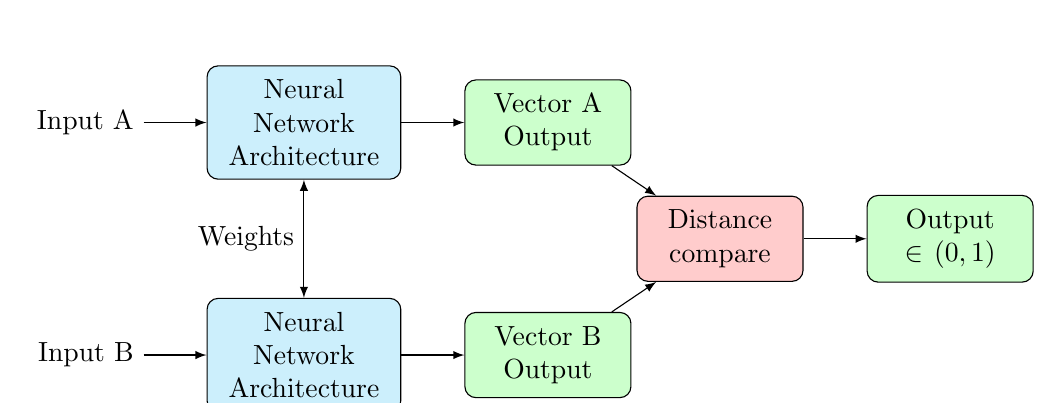
\begin{tikzpicture}[node distance = .8]
  \tikzstyle{module}=[rounded corners, draw, inner sep = 5, text width=5em, align=center]
  \tikzstyle{sister}=[module, fill=cyan!20, text width=6em]
  \tikzstyle{out-node}=[module, fill=green!20]

  \node [sister] (S-A) at (0, 0) {Neural Network Architecture};
  \node [sister, below = 1.5 of S-A] (S-B) {Neural Network Architecture};
  
  \node [left = of S-A] (I-A) {Input A};
  \node [left = of S-B] (I-B) {Input B};
  
  \node [out-node, right = of S-A] (O-A) {Vector A \\ Output};
  \node [out-node, right = of S-B] (O-B) {Vector B \\ Output};
  \node (aux-1) at ($(O-A)!0.5!(O-B)$) {};

  \node [module, right = 1 of aux-1, fill=red!20] (D) {Distance \\ compare};

  \node [out-node, right = of D] (O) {Output \(\in (0, 1) \) };

  \draw [-latex] (I-A) -- (S-A);
  \draw [-latex] (I-B) -- (S-B);

  \draw [-latex] (S-A) -- (O-A);
  \draw [-latex] (S-B) -- (O-B);

  \draw[-latex] (O-A) -- (D);
  \draw[-latex] (O-B) -- (D);

  \draw [-latex] (D) -- (O);

  \draw [latex-latex] (S-A) -- (S-B) node[midway, left] {Weights};
\end{tikzpicture}
  \caption{Siamese Network basic structure \label{fig:siamese}}
\end{figure}

\begin{figure}
  \centering
  
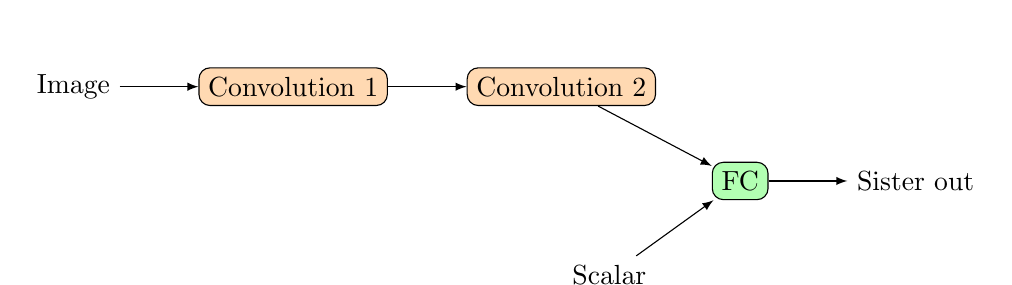
\begin{tikzpicture}[node distance = 1]

  \tikzstyle{module}=[rounded corners, draw]
  \tikzstyle{FC}=[module, fill=green!30]
  \tikzstyle{conv}=[module, fill=orange!30]

  \node [conv] (CNN-1) at (0, 0) {Convolution 1};
  
  \node [left = of CNN-1] (image) {Image};
  \node [conv, right = of CNN-1] (CNN-2) {Convolution 2};
  \node [FC, below right = of CNN-2] (FC-1) {FC};
  \node [right = of FC-1] (out) {Sister out};

  \node [below left = of FC-1] (scalar) {Scalar};


  \draw [-latex] (CNN-1) -- (CNN-2);
  \draw [-latex] (CNN-2) -- (FC-1);
  \draw [-latex] (FC-1) -- (out);

  \draw [-latex] (image) -- (CNN-1);
  \draw [-latex] (scalar) -- (FC-1);
\end{tikzpicture}



  \caption{Shallow sister network design \label{fig:shallow-sister}}
\end{figure}

This is one of the most important parts of the project, since it will have a huge
impact in the final results. It will take around four weeks to complete more or less
and it will be a trial and error process to try to see which architecture for the sister
network is best suited to solve the problem.

In this phase the designed networks will be very shallow to make small and fast improvements
since the training time could be an issue.

\sssecc{Build deep siamese network}

Once an initial shallow network is already created, then the next step will be to try 
and create a more deep version. To do so, it will be done step by step adding one layer
at a time and seeing how the network is performing.

The main advantage of deep networks against shallow networks is that they are able to
identify more complex features and thus they usually perform better. However, its 
main drawback is that training time is longer and therefore, the development process is 
slower.

\sssecc{Compare the model against other ones}

Once the final deep model is created, it will be compared against different methods of 
survival analysis. Since this method will be the first one using both image data and scalar 
data it will be compared against models using only one or the other. 

To compare the model, the \gls{CV} \gls{CI} needs to be obtained first. Afterwards,
it will be compared against models trained using the same dataset, using the 
\emph{radiomic} features extracted with PyRadiomics but using
a \gls{CPH} model instead.
~\cites{medical:py-radiomics}{medical:cox}

To do all the comparisons, the \gls{PMHNK} will be trained with each model multiple times.
That's why this task will take around to weeks to complete.

\ssecc{Estimated time}

In \autoref{tab:time} an estimation of the number of hours dedicated to each task is shown.

\begin{table}[H]
  \centering{}
  \begin{tabular}{|l|r|}
    \hline
    Task & Estimated duration (h) \\ \hline \hline
    Acquire background in CNN & 120 \\ \hline
    Get familiar with survival models & 80 \\ \hline
    Preprocess data & 40 \\ \hline
    Build shallow siamese network & 200 \\ \hline
    Build deep siamese network & 80 \\ \hline
    Compare models & 80 \\ \hline
    Final stage & 160 \\ 

  
    \hline \hline
    \textbf{Total} & 760 \\
    \hline
  \end{tabular}
  \caption{Estimated time for each task \label{tab:time}}
\end{table}

\ssecc{Gantt chart}

\autoref{fig:gantt} shows the planning of the different tasks of the project in a Gantt chart.

\begin{figure}[H]
  \centering{}
  \def\gantttext{4cm}
  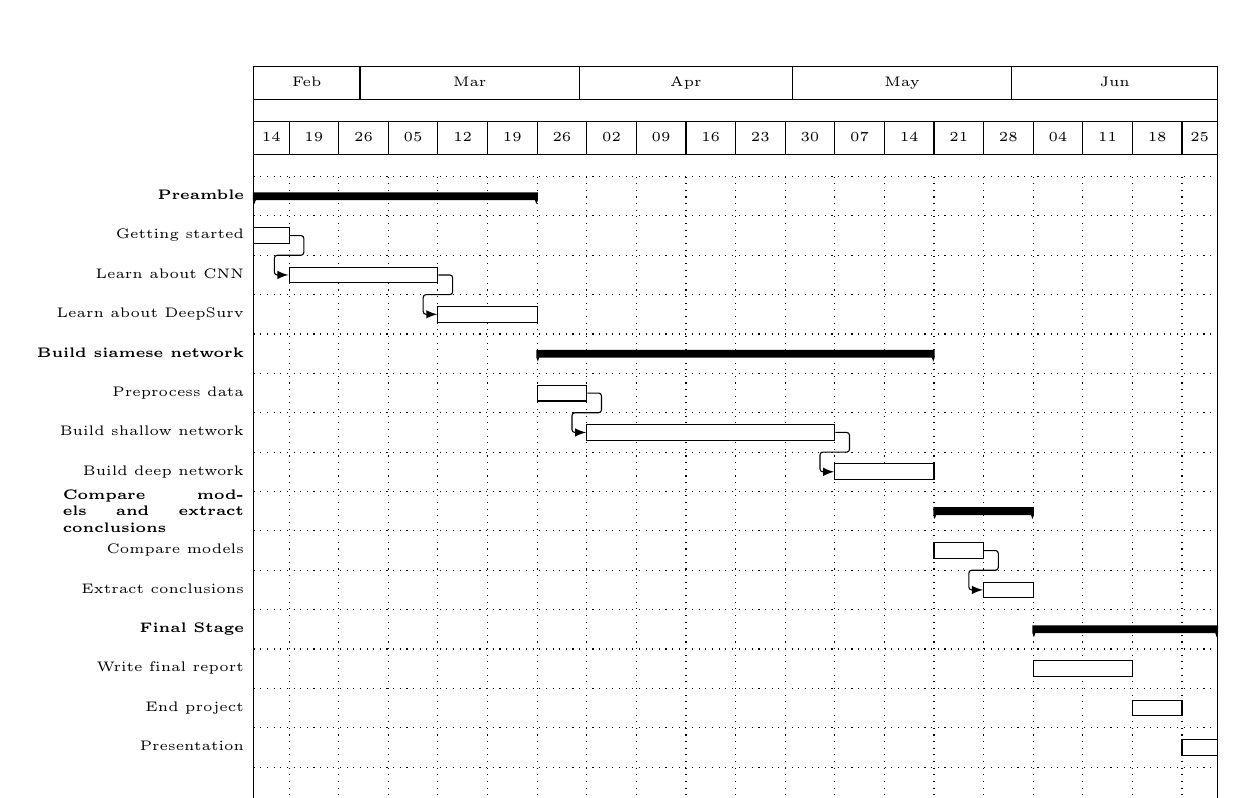
\begin{tikzpicture}
  \begin{ganttchart}[
      time slot format=isodate,
      x unit = .9mm,
      y unit title = 0.7cm,
      y unit chart = 0.5cm,
      group label font = \tiny\bfseries,
      title label font = \tiny,
      bar label font = \tiny,
      vgrid={*{4}{draw=none},dotted,*{2}{draw=none}},
      hgrid,
      calendar week text = {\startday},
      link bulge = 2,
    ]{2018-02-14}{2018-06-29}
    \gantttitlecalendar{month=shortname, week} \\


    % Start gantt itself
    \ganttgroup{Preamble}{2018-02-14}{2018-03-25} \\
    \ganttbar{Getting started}{2018-02-14}{2018-02-18} \\
    \ganttlinkedbar{Learn about CNN}{2018-02-19}{2018-03-11} \\
    \ganttlinkedbar{Learn about DeepSurv}{2018-03-12}{2018-03-25} \\

    
    \ganttgroup{Build siamese network}{2018-03-26}{2018-05-20} \\
    \ganttbar{Preprocess data}{2018-03-26}{2018-04-01} \\
    \ganttlinkedbar{Build shallow network}{2018-04-02}{2018-05-06} \\
    \ganttlinkedbar{Build deep network}{2018-05-07}{2018-05-20} \\

    \ganttgroup{\parbox[r]{2.3cm}{Compare models and extract conclusions}}{2018-05-21}
    {2018-06-03} \\

    \ganttbar{Compare models}{2018-05-21}{2018-05-27} \\
    \ganttlinkedbar{Extract conclusions}{2018-05-28}{2018-06-03} \\

    \ganttgroup{Final Stage}{2018-06-04}{2018-06-29} \\
    \ganttbar{Write final report}{2018-06-04}{2018-06-17} \\
    \ganttbar{End project}{2018-06-18}{2018-06-24} \\
    \ganttbar{Presentation}{2018-06-25}{2018-06-29} \\

  \end{ganttchart}
  \end{tikzpicture}
  \caption{Gantt chart of the project \label{fig:gantt}}
\end{figure}

\ssecc{Action plan}

As it has already been said, the fact that there will be weekly meetings will allow to 
revise and adapt the initial planning. This means that, for each task, the real duration, 
compared to the planned one may differ, and thus the planning will be changed accordingly. 
If a task is finished before planned, then the next task will start immediately. 
Moreover, if a task duration is longer than expected, then the following tasks will need 
to be rescheduled or, in the worst case, omitted, although not all the tasks can be excluded.

Having weekly meetings with the Principal Investigator should mitigate the possible problems,
and give enough time to detect possible delays or differences with the original time. Therefore,
I should be able to fix them as soon as they are detected.

Below, there are some examples of potential sources of delays.

\sssecc{Complexity of the built model}

Since the model that it's going to be built is quite complex, it will have a constant trial
and error. This can cause delays if a wrong architecture it's chosen, and it's not detected
on time, because a lot of time can be lost trying to optimize a wrong model,
until it's noticed. 

\sssecc{Bugs}

Using complex software such as Tensorflow is prone to errors in many ways. Programming errors
are not an exception and while writing the code some bugs can be introduced. If a bug is not 
noticed soon, it can cause long delays while trying to fix them.

\sssecc{Unavailability of \acrlong{CC}}

Since this project involves training \glspl{CNN}, it needs a lot of computing 
power so \gls{CC} computing cluster will be used to train the data. If the cluster it's not available,
then the training will need to be done with local resources which will be slower and thus 
more time will be lost.

\sssecc{Training times}

The training time is one of the biggest drawbacks of this project. Since this task
can take a huge amount of time depending on the chosen architecture it can cause
huge delays in the original plan. This should be mitigated by doing small tests
instead of a whole training session to make sure that no bugs are found in the code 
because, otherwise, all the training results would become invalid.

\ssecc{Project budget \label{sec:budget}}

In order to carry out this project some resources will be needed. In this document, 
an estimation of the cost of the project is presented, keeping in mind the required
hardware and software resources, and its corresponding amortizations. Also, the
indirect costs of the project are counted too.

\sssecc{Hardware budget}

In order to implement the different models previously explained, some hardware will be
needed. The training will usually be done in Compute Canada computing platform. The
access to the different provided clusters it's provided by the Bioinformatics and 
Computational Genomics Laboratory.

\autoref{tab:hardware-budget} shows an estimation of the cost of the hardware used in the
project, taking into account its useful life and its amortizations.

\begin{table}[H]
  \centering
  \begin{tabular}{|l|r|r|r|r|}
    \hline
    \textbf{Product} & \textbf{Price} & \textbf{Units} & \textbf{Useful life} 
    & \textbf{Amortization} \\ \hline\hline

    MSI GL62M 7RD-429XES & 1.000 € & 1 & 5 years & 83 € \\ \hline
    Lab iMac & 0 € & 1 & -- & 0 € \\ \hline
    Compute Canada platform & 0 € & 1 & -- & 0 € \\ \hline

    \hline\hline
    \textbf{Total} & 1.000 € & \multicolumn{2}{|c|}{} & 83 € \\ \hline
  \end{tabular}
  \caption{Hardware budget \label{tab:hardware-budget}}
\end{table}

\sssecc{Software budget}

Some software will be used to carry out the project. Since this project will be used using
Open Source and free tools the total software cost of the project is zero. 
\autoref{tab:software-budget} shows an estimation of the cost of the software used in the 
project.

\begin{table}[H]
  \centering
  \begin{tabular}{|l|r|r|r|}
    \hline
    \textbf{Product} & \textbf{Price} & \textbf{Units} & \textbf{Amortization} \\ \hline\hline

    Python & 0 € & 1 & 0 € \\ \hline
    Tensorflow & 0 € & 1 & 0 € \\ \hline
    PyDicom & 0 € & 1 & 0 € \\ \hline
    NumPy & 0 € & 1 & 0 € \\ \hline
    Scikit & 0 € & 1 & 0 € \\ \hline
    Visual Studio Code & 0 € & 1 & 0 € \\ \hline
    Git & 0 € & 1 & 0 € \\ \hline
    GitHub & 0 € & 1 & 0 € \\ \hline
    PyCharm Community Edition & 0 € & 1 & 0 € \\ \hline
    \LaTeX & 0 € & 1 & 0 € \\ \hline
    Vim & 0 € & 1 & 0 € \\ \hline

    \hline\hline
    \textbf{Total} & 0 € &  & 0  € \\ \hline
  \end{tabular}
  \caption{Software budget \label{tab:software-budget}}
\end{table}


\sssecc{Human resources budget}

To develop this software some roles will be taken. There will be the Project Manager role,
the Software Developer role and the Tester role. Each role is differentiated in the total
of 760 hours. \autoref{tab:salary} shows the estimated costs for each role and the
Human Resources cost, \autoref{tab:time-estimation} shows an estimation of the time 
inverted on each role for each task.

\begin{table}[H]
  \centering
  \begin{tabular}{|l|r|r|r|}
    \hline
    \textbf{Role} & \textbf{Hours} & \textbf{€/hour} & \textbf{Salary} \\ \hline\hline

    Project Manager & 70 & 33,8 & 2.366 € \\ \hline
    Software Developer & 510 & 23,4 & 11.914 € \\ \hline
    Tester & 180 & 19,5 & 3.510 € \\ \hline

    \hline\hline 
    Total & 760 & & 17.810 € \\
    \hline
  \end{tabular}

  \caption[Human Resources budget]{
    Human resources budget, salary according to \cite{ine:salary} \label{tab:salary}
  }
\end{table}

\begin{table}[H]
  \centering
  \begin{tabular}{|P{4cm}|r|r|r|r|}
    \hline
    \multirow{2}{*}[-1em]{\textbf{Task}} & 
    \multirow{2}{*}[-1em]{\textbf{Duration}} & 
    \multicolumn{3}{|c|}{\textbf{Dedication}} \\ \cline{3-5}

     & & \parbox[c][1.5cm]{2.1cm}{\textbf{Project \\ Manager}} & 
     \parbox[c][1.5cm]{2.2cm}{\textbf{Software \\ Developer}} & 
     \textbf{Tester} \\ \hline\hline

     Acquire background in CNN & 120 & 10 & 110 & 0 \\ \hline
     Get familiar with survival models & 80 & 10 & 70 & 0 \\ \hline
     Preprocess data & 40 & 10 & 20 & 10 \\ \hline
     Build shallow siamese network & 200 & 15 & 110 & 75 \\ \hline
     Build deep siamese network & 80 & 10 & 50 & 20 \\ \hline
     Compare models & 80 & 10 & 40 & 30 \\ \hline
     Final stage & 160 & 5 & 110 & 45 \\ 

     \hline\hline
     \textbf{Total} & 760 & 70 & 510 & 180 \\
     \hline
  \end{tabular}

  \caption{Time estimation by role \label{tab:time-estimation}}
\end{table}

\sssecc{Unexpected costs}

As there may be unexpected changes in the project, an extra budget has to be added to compensate
for such problems. \autoref{tab:unexpected-costs} shows the distribution of this budget per role.

\begin{table}[H]
  \centering
  \begin{tabular}{|l|r|r|r|}
    \hline
    \textbf{Role} & \textbf{Hours} & \textbf{€ / hour} & \textbf{Salary} \\ \hline\hline
    Project Manager & 10 & 33.8 & 338 € \\ \hline
    Software Developer & 20 & 23.4 & 468 € \\ \hline
    Tester & 10 & 19.5 & 195 € \\ \hline

    \hline\hline
    \textbf{Total} & 40 & & 1001 € \\ 
    \hline
  \end{tabular}
  \caption{Unexpected costs \label{tab:unexpected-costs}}
\end{table}

\sssecc{Indirect costs}

In a project, there are some costs that cannot be added in neither of the previous categories,
this are estimated in \autoref{tab:indirect-costs}.

\begin{table}[H]
  \centering
  \begin{tabular}{|l|r|r|r|}
    \hline
    \textbf{Product} & \textbf{Price} & \textbf{Units} & \textbf{Cost} \\ \hline\hline

    Electricity & 0,12 €/kWh & 550 kWh & 66 € \\ \hline
    Internet + phone & 70 €/month & 4 months & 280 € \\ \hline
    
    \hline\hline
    \textbf{Total} & & & 346 € \\ \hline
  \end{tabular}
  \caption{Indirect costs \label{tab:indirect-costs}}
\end{table}

\sssecc{Total budget}

By adding all the previously provided budgets, the total estimated budget for this project
is obtained, as shown in table \autoref{tab:total-costs}. Notice that a 5\% of contingency
has been added over the cumulative total in order to cover unexpected expenses that may 
occur during the development of the project.

\begin{table}[H]
  \centering
  \begin{tabular}{|l|r|}
    \hline
    \textbf{Concept} & \textbf{Estimated Costs} \\ \hline\hline

    Hardware resources & 83 € \\ \hline
    Software resources & 0 € \\ \hline
    Human resources & 17.810 € \\ \hline
    Unexpected costs & 1001 € \\ \hline
    Indirect costs & 346 € \\ \hline

    \hline\hline
    \textbf{Subtotal} & 19.240 € \\
    \hline\hline
    Contingency (5\%) & 962 € \\
    \hline\hline
    \textbf{Total} & \textbf{20.202 €} \\ \hline
  \end{tabular}

  \caption{Total project costs \label{tab:total-costs}}
\end{table}

Finally, an estimation of the approximate budget per task is also provided in 
\autoref{tab:task-cost}. The cost of each task is computed using the number of hours spent 
in the task and the required resources.

\begin{table}[H]
  \centering
  \begin{tabular}{|l|r|}
    \hline
    \textbf{Task} & \textbf{Estimated cost} \\ 
    \hline\hline

    Acquire background in CNN & 3.189,79 € \\ \hline
    Get familiar with survival models & 2.126,53 € \\ \hline
    Preprocess data & 1.063,26 € \\ \hline
    Build shallow siamese network & 5.316,32 € \\ \hline
    Build deep siamese network & 2.126,53 € \\ \hline
    Compare models & 2.126,53 € \\ \hline
    Final stage & 4,253.05 € \\ 

    \hline\hline
    \textbf{Total} & 20.202,00 € \\ \hline
  \end{tabular}

  \caption{Project's tasks costs \label{tab:task-cost}}
\end{table}

\ssecc{Budget control}

Controlling the spent budget is a very important part of the project. Using too much time or 
having to buy unexpected hardware could be a problem but it's likely to happen. That's why
some plans will be made to avoid, as much as possible, this situation.

It may be necessary to buy extra software or to have more human resources although it's
unlikely that it may be necessary more hardware. Solving the extra software requirement
shouldn't be a big problem as there are many free or open source software solutions in
the market.

To control the human resources budget, the number of hours working as each role will be 
recorded, this way then it can be seen if too much time has been used for a task and then
it can be solved by rescheduling the next tasks.

\ssecc{Sustainability and social commitment}

In order to evaluate the project's sustainability, environmental impact will be analyzed
regarding three major factors: environmental, social and economical. The analysis will be 
based in the application of the sustainability matrix to the project shown in
\autoref{tab:sustainability} and in the poll that can be accessed through 
\url{https://goo.gl/kWLMLE}.

\begin{table}[H]
  \centering
  \begin{tabular}{|c|c|c|c|}
    \cline{2-4}
    \multicolumn{1}{c|}{} & \textbf{PPP} & \textbf{Useful life} & \textbf{Risks} \\ 
    \hhline{-===}

    \multirow[c]{2}{*}{\textbf{Environmental}} & 
    \makecell{Design \\ consumption} & \makecell{Ecological \\ footprint} & 
    \makecell{Environmental \\ risks} \\ \cline{2-4}
    & 2/10 & 19/20 & -2/-20 \\ \hline
    
    \multirow{2}{*}{\textbf{Economical}} & 
    Bill & \makecell{Viability \\ plan} & \makecell{Economical \\ risks} \\ \cline{2-4}
    & 7/10 & 18/20 & -15/-20 \\ \hline

    \multirow{2}{*}{\textbf{Social}} &
    \makecell{Personal \\ impact} & \makecell{Social \\ Impact} & 
    \makecell{Social \\ risks} \\ \cline{2-4} 
    & 9/10 & 18/20 & -5/-20 \\ \hline

    \hline\hline
    \multirow{2}{*}{\parbox[c]{3cm}{\centering\textbf{Sustainability \\ range}}} &
    18/30 & 55/60 & -22/-60 \\ \cline{2-4}
    & \multicolumn{3}{c|}{51/90} \\ \hline

  \end{tabular}
  \caption{Project's sustainability matrix \label{tab:sustainability}}
\end{table}

\sssecc{Evaluation}

Nowadays sustainability is a great issue, the progress made by humanity in the technology
field it has some consequences too. Information and Communication Technologies are not 
an exception although it has taken some time to gain importance. The appearance of 
small devices like smartphones and the huge power requirements of big data centers have 
helped in gaining conscience of power consumption. 

When trying to build a new project now it's important to see project's sustainability. If the
project involves building some hardware then it may have a negative impact on the environment
so proper measures need to be taken to avoid future problems.

Moreover, if the project it's software related then it has some implications too. In general
when working with this type of projects the only part where it can be a problem is regarding
power consumption, which is usually related to efficiency. As a general rule they should
avoid using too much power but it depends on the project's type. Machine Learning ones
usually have a big power consumption during the training phase since it requires a huge
amount of computational power. However, smartphone related applications tend to have less
consumption to allow for a longer battery life.

However, regarding the budget, solutions that tend to be more sustainable usually are more
expensive. When it is attempted to reduce consumption in software projects, this usually 
translates in more programmer hours and thus a higher budget.

\sssecc{Environmental dimension}

Regarding the environmental dimension the project has two main stages. Since the main objective
of the project is to develop a deep learning model the first stage is to create the model
itself. The second one is to deploy the product and start using it.

In the first stage many resources will be needed since the training process in machine learning
requires a huge amount of computational power. This is directly translated to electricity 
consumption so, during the development process the environmental impact will be hight.

However, once a model is already trained, using it does not require much power since the
data inference it's quite fast and thus, does not require many electricity consumption.
That's why the second part of the project won't have a very hight environmental impact.

\sssecc{Social dimension}

As there is a lot of research regarding this topic, creating this project should help pushing 
forward the development of new methods for survival analysis. Either if the project results 
are positive or negative it should help to prove that a certain method is valid or not. 

In addition, it's primary focus is medical, so it's very social oriented. Thus,
in the long term, it should help cancer patients to receive better treatments 
that will be developed with help of survival analysis models. 

Regarding the personal and ethical implications, it will help having a better understanding
of machine learning models, how to use them and how to develop them. Moreover, this project
will not have any ethical issue but the contrary, knowing that the social outcome can be
positive it's an incentive to work and do a good job.

\sssecc{Economical dimension}

A detailed exposition of all the related project costs has already been made including both
human and material resources, as shown in \autoref{sec:budget}.

This project should have a positive impact regarding the economical dimension. Improving
the methods for survival detection helps reducing the costs of future research. However, 
there's the downside that if the research has some kind of mistake that it's not noticed,
a negative impact may occur due to the fact that some related researches may have to roll
back some results.

\ssecc{Laws and regulations}

As this project uses patient's information from \gls{UHN}, it's subject of Ontario's (Canada)
regulations and \gls{UHN}'s policies regarding privacy protection.

Ontario's \gls{PHIPA} defines patient's privacy rights and the ways that their 
\gls{PHI} may be handled. \gls{PHIPA} builds on other laws in setting out the rules
to protect patient information. \gls{PHI} is information that identifies the person
and connects that person to receiving care at the hospital.

\gls{UHN}'s privacy policy states that a patient's privacy and proper use of personal health 
information must be ensured. All the patient's \gls{PHI} must be treated with respect
and sensitivity. Moreover, data should be de-identified whenever possible and always
before sending \gls{PHI} to an unauthorized recipient or presenting findings in a 
presentation or publication
~\cite{medical:uhn:policies:privacy}.

\gls{UHN}'s confidentiality agreement ensures that I follow the privacy policies, as I 
can have access to information and material relating to patients, medical staff, employees,
or UHN which is private and confidential
~\cite{medical:uhn:agreement:confidentiality}. 



\cleardoublepage
% % !TEX root = ../main.tex

\addtocontents{toc}{\protect\newpage}
\secc{Design and implementation}

\ssecc{Get familiar with survival models}

\ssecc{Preprocess data}

As it was previously stated the data needs to be preprocessed before start training with it.
This steps are required because small changes can really help in reducing the time needed to
fit the model. Also, by normalizing the data and setting variance to 1 and mean to 0 the network
can converge faster.
~\cite{neural:efficient-backprop}

The whole preprocess task took longer than expected as many tasks required more steps than 
planned. The planned duration was 1 week and the final duration was from March 13\Th and
ended in April 11\Th so its duration was of 4 weeks. However, this wasn't as problematic as 
it could seem since the previous task was completed early.

Also, this task has been done sometimes while doing other tasks because some preprocess 
steps have been added later to improve the network's results.

\sssecc{Image data}

The imaging data in the \Gls{PMHNK} contains 671 folders, each one with the scan of one patient. 
We also have the clinical information of 661 patients, although we do not have a \gls{CT} for
each of the clinical information patients. Through the intersection of each of the two data
sources we have 544 patients with both a \gls{CT} scan and the clinical information.

However, because there was a problem in the way the \gls{CT} scan was computed we only have
the tumour annotations for 509 of the 544 patients, so the data that we can use is reduced
again. \textbf{509} will be the final dataset size that will be used for the next 
steps.

For all the valid patients their directory structure is the same. They contain two folders,
one with all the original scan slices and the other with the slice's tumour mask annotations. 
All the slices are in \verb|.dcm| format.
As an example, the structure for patient \texttt{FHBO0003} can be seen in \autoref{fig:hnk-raw}.

\begin{figure}
  \centering
  \begin{minipage}{0.8\textwidth}
    \begin{Verbatim}[samepage=true]
FHBO003
├── FHBO003           // Original scan
│   ├── IMG0001.dcm
│   ├── IMG0002.dcm
│   ├── ...
│   └── IMG0191.dcm
└── FHBO003-MASS      // Annotated mask
    ├── IMG0001.dcm
    ├── IMG0002.dcm
    ├── ...
    └── IMG0191.dcm
    \end{Verbatim}
  \end{minipage}
    
  \caption{Original data directory structure \label{fig:hnk-raw}}
\end{figure}

Preprocessing the image data requires multiple steps:
\begin{enumerate}
  \item Select valid directories that follow the previously stated conditions
  \item Join all the \verb|.dcm| files into a 3D \verb|numpy| array
  \item Apply gaussian filter to mask image. This is done because the mask is manually annotated
        and usually each layer does not fit perfectly with the previous one. This way a smooth
        transition between layers is ensured.
  \item Get 3D bounding box containing the tumour.
  \item Slice original image and mask with the bounding box to extract the parts only containing
        the tumour. A single bounding box is obtained.
  \item Remove extreme values, if the value of the image is smaller than -1000 or bigger than
        400 this means that this are pixels usually outside of the scanner. This happens because
        the scanner has a circular field of view but a squared image is generated instead, so 
        all the pixels outside the circle are \emph{error pixels}.
  \item Apply mask to extracted image. Since the mask only contains 1s and 0s it's as easy 
        as \verb|image *= mask|.
  \item Resize the sliced image to a size of \( 64 \times 64 \times 64 \)
  \item Normalize image by setting mean = 0 and variance = 1. It's done in the following way:
  \begin{itemize}
    \item \verb|image -= mean(image)|
    \item \verb|image /= std(image)|
  \end{itemize}
  \item Rotate the image 3 times to get 4 different versions of the scan that can be used for 
        training as data augmentation.
\end{enumerate}

\begin{figure}
  \resizebox{\textwidth}{.7\textwidth}{
    \def\customimage{5em}
\begin{tikzpicture}[node distance = 2]
    \node (P-0) at (0, 0) {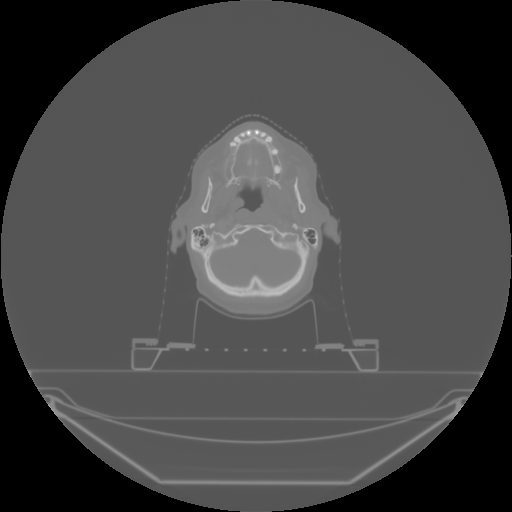
\includegraphics[width=\customimage]{images/preprocess/process_0}};
    \node [below = of P-0] (P-1) {
\includegraphics[width=\customimage]{images/preprocess/process_1}};

    \node [below = .2 of P-0] (text-0) {Scan};
    \node [below = .2 of P-1] (text-1) {Mask};
    
    \node [right = of P-1] (P-2-0) {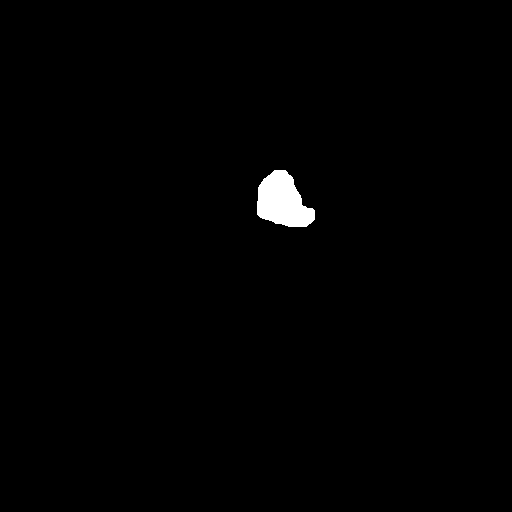
\includegraphics[width=\customimage]{images/preprocess/process_2_0}};
    \node [right = of P-2-0] (P-2-1) {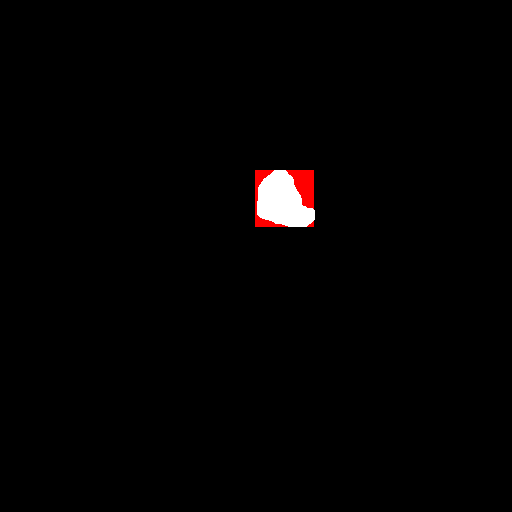
\includegraphics[width=\customimage]{images/preprocess/process_2_1}};
    \node [right = of P-2-1] (P-5) {
\includegraphics[width=\customimage]{images/preprocess/process_5}};
    
    \node [above = of P-2-1] (P-3) {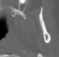
\includegraphics[width=\customimage]{images/preprocess/process_3}};
    \node [right = of P-3] (P-4) {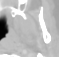
\includegraphics[width=\customimage]{images/preprocess/process_4}};

    \node [right = .5 of P-5, circle, draw] (prod) { \Large \( \times \) };
    
    \node [below = of P-5] (P-6) {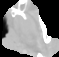
\includegraphics[width=\customimage]{images/preprocess/process_6}};
    \node [left = of P-6] (P-7) {
\includegraphics[width=\customimage]{images/preprocess/process_7}};
    \node [left = of P-7] (P-8) {
\includegraphics[width=\customimage]{images/preprocess/process_8}};

    \node [below = .2 of P-6] { \( 59 \times 57 \) px};
    \node [below = .2 of P-7] { \( 64 \times 64 \) px};
    \node [below = .2 of P-8] { \( 64 \times 64 \) px};

    \draw [-latex] (P-0) -- (P-3);
    \draw [-latex] (P-3) -- (P-4) node[midway, below, align=center] {Remove \\ extreme \\ values};
    \draw [-latex] (P-4) -| (prod);

    \draw [-latex] (P-1) -- (P-2-0) node[midway, below, align=center] {Gaussian \\ filter};
    \draw [-latex] (P-2-0) -- (P-2-1) node[midway, below, align=center] {Bounding \\ box};
    \draw [-latex] (P-2-1) -- (P-3) node[midway, right, align=center] {Slice};
    \draw [-latex] (P-2-1) -- (P-5) node[midway, below, align=center] {Slice};
    \draw [-latex] (P-5) -- (prod);

    \draw [-latex] (prod) |- (P-6) node[near end, below, align=center] {Apply \\ mask};
    \draw [-latex] (P-6) -- (P-7) node[midway, below, align=center] {
        Resize \\ \( 64 \times 64 \)
    };

    \draw [-latex] (P-7) -- (P-8) node[midway, below, align=center] {Normalize};

\end{tikzpicture}
  }

  \caption[Image pre-process pipeline]{
    Image pre-process pipeline \label{fig:preprocess}
    
    In this example the process is shown for a 2D image, all the pictures are being resized to 
    have the same size so the steps can be appreciated. The normalization step is not shown as is,
    since setting a mean of 0 and variance of 1 produces an invalid \acrshort{PNG} image, but still valid
    for \gls{ML} purposes.
  }
\end{figure}

\sssecc{Scalar data}

There are two types of scalar data:
\begin{itemize}
  \item Clinical information
  \item Radiomic features extracted from the image, regarding tumour shape, intensity, volume...
\end{itemize}

The clinical information should be anonymized as much as possible and especially if it's going
to be outside \gls{UHN}, the network of hospitals where this project is being developed.
Since this is the case, as the training will be done at \gls{CC} cluster, the unnecessary fields
are removed and only those being used are kept. Moreover, removing the unused fields
is helpful when using the data.

Originally, the clinical information provides 36 different fields. From these fields only the 
following ones are kept:
\begin{itemize}
  \item ID
  \item Age
  \item Sex
  \item Survival event. This one needs to be negated since, in the provided event, \verb|event = 1|
        means survival, but in our survival model this means death. 
  \item Survival time
\end{itemize}

The radiomic features can be extracted directly with the \emph{PyRadiomics}
\cite{medical:py-radiomics} package, but in this case they have been already extracted and stored
in a single file so we can reuse them. These features should be normalized before start training,
because otherwise the network may never converge, which indeed it happened. 

For this normalization to be valid, the mean and the standard deviation are obtained only from 
the train samples. These are different for each feature because not all the features need to 
be normalized in the same way. Afterwards, the normalization is applied to both the train 
and test samples. The mean for the test samples is never obtained, because, otherwise, the
model could have \gls{leakage}. An example of features normalization can be seen in
\autoref{fig:feature-normalization}

\begin{figure}
  \centering

  \begin{subfigure}[t]{.49\textwidth}
    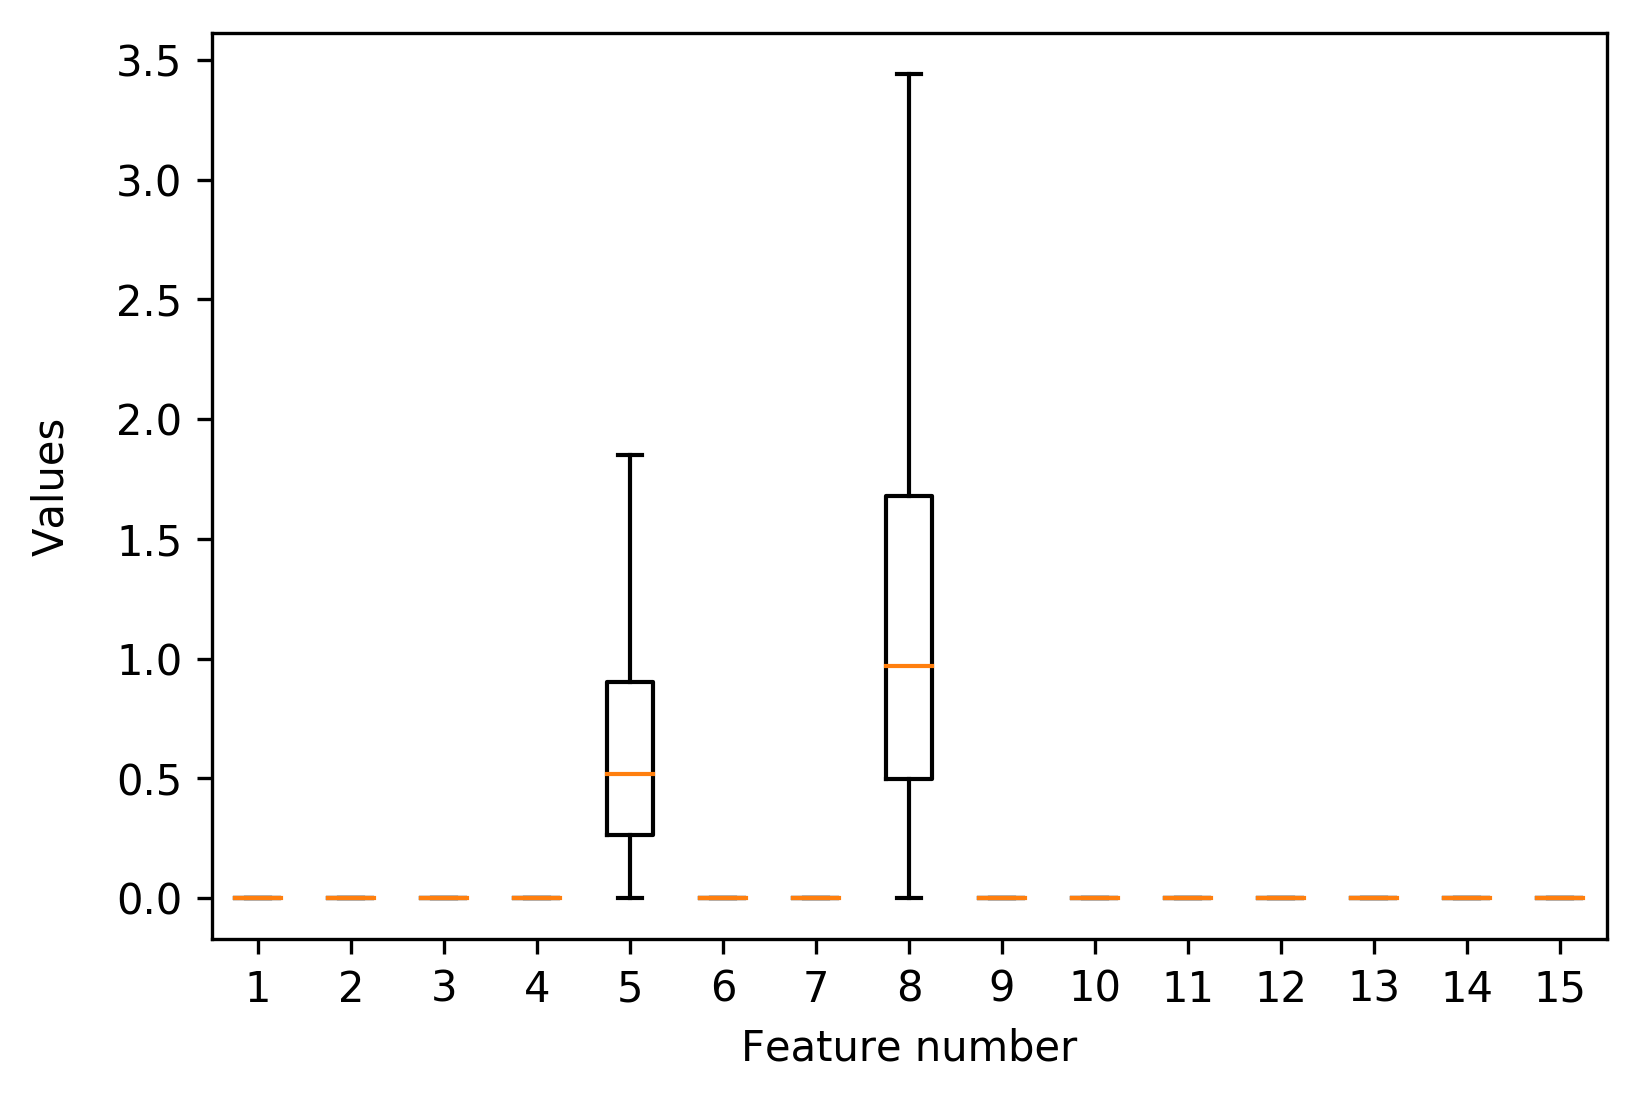
\includegraphics[width=\textwidth]{images/features_original}

    \caption{Features' box plot before normalization \label{fig:feature-normalization-before}}
  \end{subfigure}
  \hfill
  \begin{subfigure}[t]{.49\textwidth}
    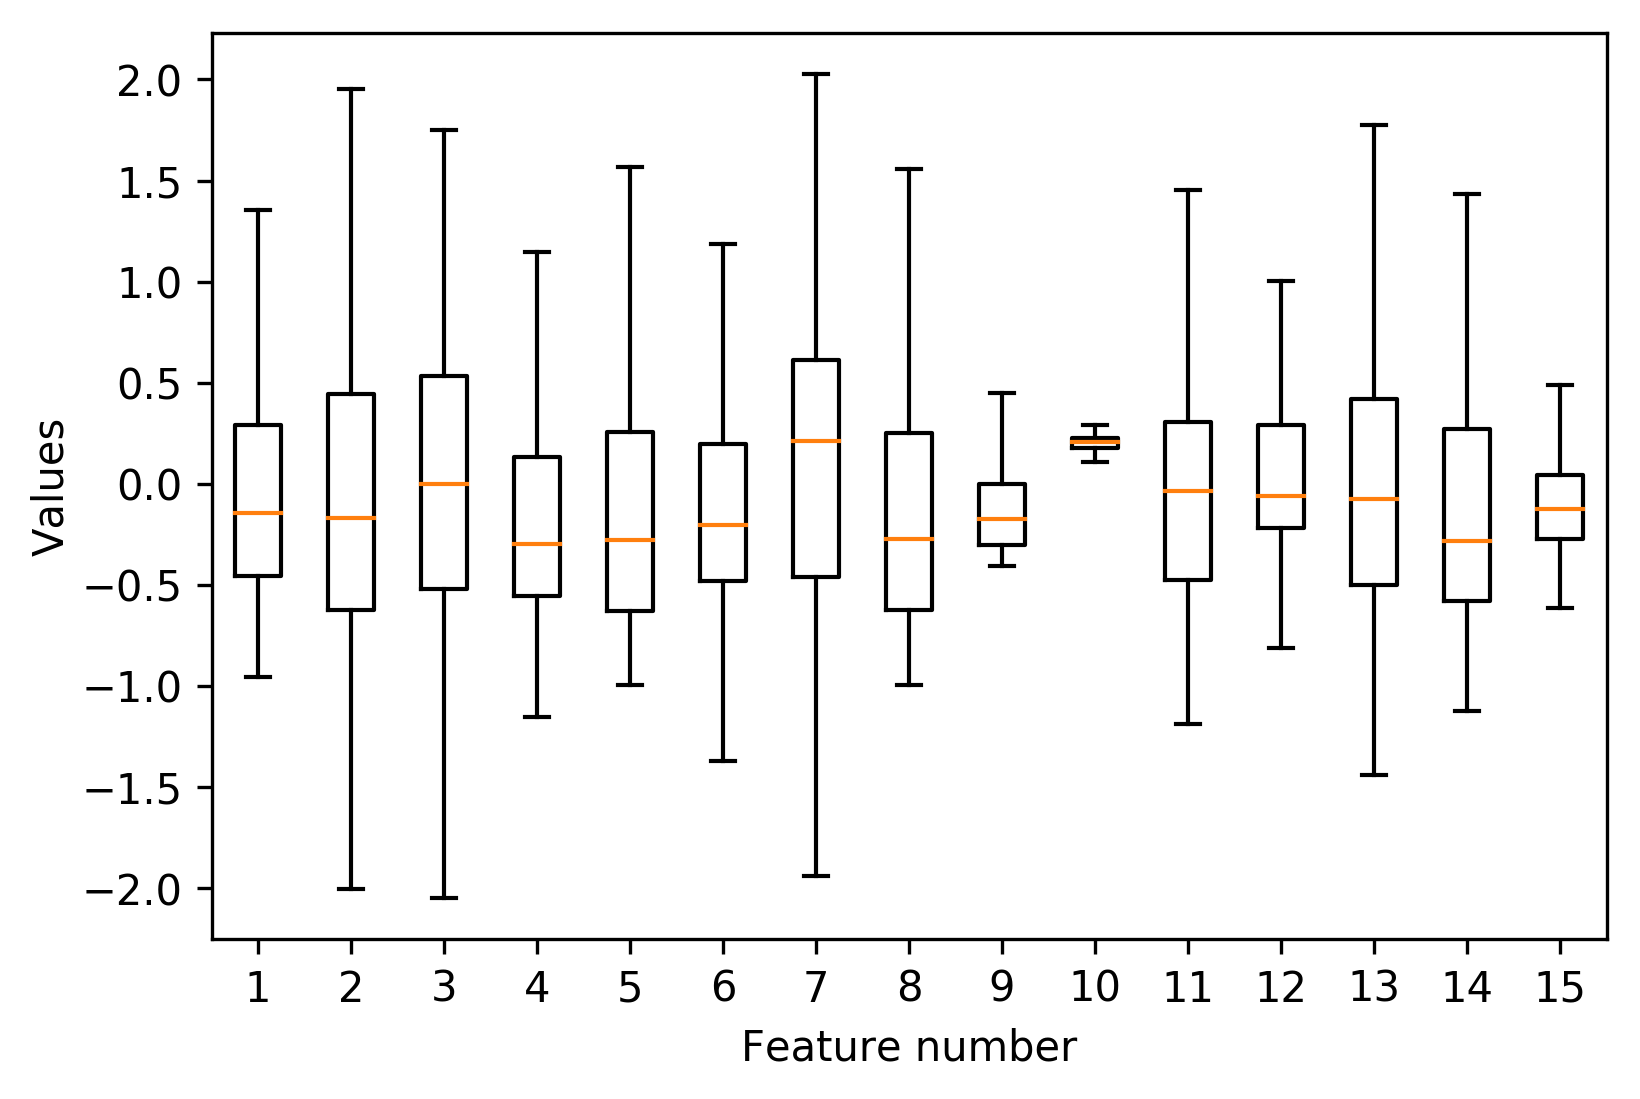
\includegraphics[width=\textwidth]{images/features_normalized}

    \caption{Features' box plot after normalization}
  \end{subfigure}

  \caption[Features normalization example]{
    Features normalization example \label{fig:feature-normalization}
    
    In this example only the first 15 of 725 features are shown for readability. 
    \autoref{fig:feature-normalization-before} shows the features before normalizing them. 
    There, many of the features are too small compared with the ones shown so only a small 
    line is drawn.
  }
  
\end{figure}


\sssecc{Pair generation}

As the siamese network is prepared to train in pairs these have to be generated before. As
it has been explained in \autoref{sec:survival} and shown in \autoref{fig:graph-ci},
for two subjects \( A \) and \( B \) a pair can only be generated if:
\begin{itemize}[noitemsep, topsep=0pt]
  \item Both of them are uncensored (\( E_A = E_B = 1\))
  \item The uncensored time of one is smaller than the censored survival time of the other
  (\( T_A < T_B | E_A = 1; E_B = 0 \))
\end{itemize}

These conditions are to be kept in mind when generating the pairs. Moreover, before starting
the train and test sets must be decided first. Once they have been generated then the pairs
can be generated too. To avoid \gls{leakage} three types of pairs will be defined and will be
used in different contexts:
\begin{description}
  \item[\Gls{train-pair}] \glsdesc*{train-pair}
  \item[\Gls{test-pair}] \glsdesc*{test-pair}
  \item[\Gls{mixed-pair}] \glsdesc*{mixed-pair}
\end{description}

When generating mixed pairs the rules are a bit different. Since the network is not supposed
to know anything about the test set elements, only uncensored elements from the train set
are used to avoid creating pairs where both elements are censored.

\begin{figure}
  \centering
  \def\customimage{5em}
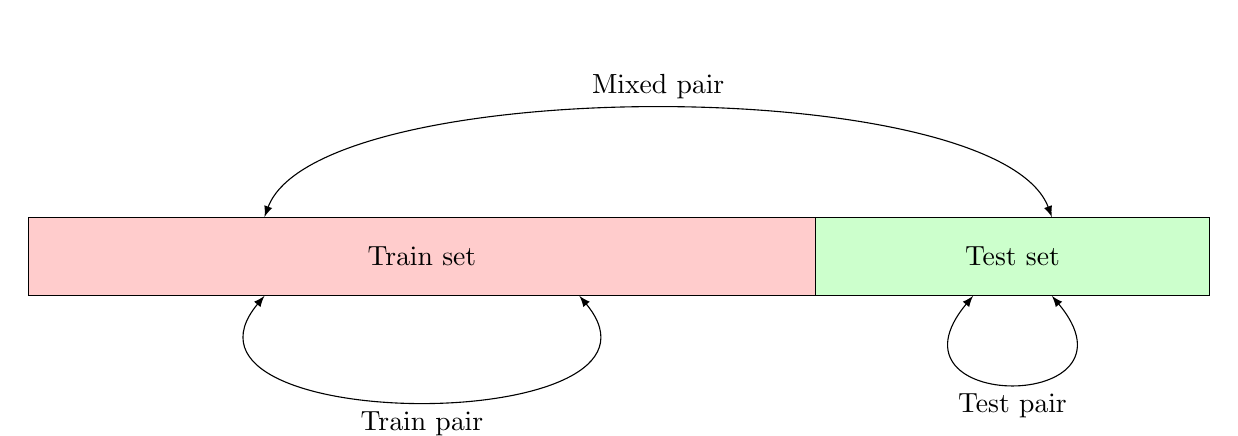
\begin{tikzpicture}
    
    \draw [fill = red!20] (0, 0) rectangle (10, 1);
    \draw [fill = green!20] (10, 0) rectangle (15, 1);

    \node at (5, .5) {Train set};
    \node at (12.5, .5) {Test set};

    \draw [bend right=130, latex-latex, looseness=1.5] (3, 0) to node [midway, below] {Train pair} (7, 0);
    \draw [bend right=130, latex-latex, looseness=5] (12, 0) to node [midway, below] {Test pair} (13, 0);
    \draw [bend left=70, latex-latex, looseness=.5] (3, 1) to node [midway, above] {Mixed pair} (13, 1);
\end{tikzpicture}
  \caption{Types of pairs generated from the test and train sets}
\end{figure}


\ssecc{Create basic siamese model}
\label{sec:basic-siamese}

The first step is to create an environment where different sisters networks can be tested
for improvements. To do so, the loss and cost functions are defined assuming a sister
network's output \( \bm{O} \) form the input \( \bm{X} \). This will be called the
\emph{basic model}.

The distance comparison used for the following siamese networks is defined comparing the 
absolute distance of the sister's output features and then applying the logistic function 
into it to get an output value \( d \in [0, 1] \). This way if it's 1 it means \( T_B > T_A \).
Future designs should implement the sister network's part for this model to work.
\begin{align*}
  \bm{O}_A &= \operatorname{sister}(\bm{X}_A) \\
  \bm{O}_B &= \operatorname{sister}(\bm{X}_B) \\
  \sigma(x) &= \frac{1}{1 + \exp(-x)} \\
  d &= \sigma(||\bm{O}_B||_2 - ||\bm{O}_A||_2) 
\end{align*}

Note that, since the output is a real number, to compute the \gls{CI} a threshold has been
set to round the real numbers to 0 or 1. The threshold value is 0,5 so if a number is 
bigger than the threshold it will be rounded to 1 and if not, it will be rounded to 0.
This conversion is only performed to compute the \gls{CI} and not when training the network.

The loss function used for the model is the log-loss:
\[
  \mathcal{L}(\bm{y}, \hat{\bm{y}}) = -\frac{1}{N} \sum_{i = 1}^{N}
  (1 - y_i)\log(1 - \hat{y}_i) + y_i\log(\hat{y}_i)
\]

The model uses L2 regularization, so the model's cost function, 
adding the regularization loss, is:
\[
  C(\bm{y}, \hat{\bm{y}}) = \mathcal{L}(\bm{y}, \hat{\bm{y}}) + 
  ||\bm{w}||_2
\]

This step was not included in the planning but it was later found that it was necessary to be 
able to test multiple models. The whole process took one week to complete.

\ssecc{Build volume only model}

To be able to have a baseline and compare the results, not only with the state-of-the art ones
but with future designs too, a model using only the most prognostic feature, the volume, is 
built.

This design is a siamese network too implementing the sister network part. The model to fit
is inspired by the idea "A bigger tumour volume means less chances of survival" 
and it is the following one:
\[
  \operatorname{sister}(x) = w\cdot x + b
\]
Where \( x \) in this case is only the volume. This model is built only to set a 
baseline for improvement.

This step was not included in the planning but having a baseline was required to see the 
improvement of the new models compared against this one. This step took half a week to complete,
including the time to test and obtain the results.

\sssecc{Results}

The results have been obtained using both 4-CV and \gls{LOOCV}. The parameters used to 
train the model have been:
\begin{itemize}
  \item Learning rate: 0,05
  \item Number of epochs: 200
  \item Batch size: The whole dataset
\end{itemize}

As seen in \autoref{tab:results-volume-4CV}, when using 4-CV. The final \gls{CI} with mixed pairs
is 0,613 and 0,623 for the test pairs.

\begin{table}
  \centering
  \begin{tabular}{|c||c|c|c||c|c|c|}
    \cline{2-7}
    \multicolumn{1}{c|}{} & \multicolumn{3}{|c||}{\textbf{Pairs}} & 
    \multicolumn{3}{c|}{\textbf{Concordance Index}} \\
    \hline
    \textbf{Fold} & \textbf{Mixed} & \textbf{Train} & \textbf{Test} 
    & \textbf{Mixed} & \textbf{Train} & \textbf{Test} \\
    \hhline{=======}
    0 & 16.359 & 46.804 & 5.330 & 0,627 & 0,634 & 0,639 \\
    1 & 16.359 & 46.957 & 5.278 & 0,629 & 0,635 & 0,63 \\
    2 & 16.348 & 47.577 & 5.084 & 0,636 & 0,627 & 0,661 \\
    3 & 16.348 & 47.274 & 5.176 & 0,618 & 0,644 & 0,6 \\
    \hhline{=======}
    \textbf{Total} & 65.414 & 188.612 & 20.868 & 0,627 & 0,635 & 0,632 \\
    \hline
  \end{tabular}

  \caption[Volume Only 4-CV results]{
    Results for volume only model using 4-CV \label{tab:results-volume-4CV}
  }
\end{table}

The results obtained with \gls{LOOCV} are shown in \autoref{fig:results-volume-LOOCV}. 
To train this model one element has been removed from the dataset and the model has 
been trained with the rest of the elements (all minus one). It shows the \gls{CI} of each
element when comparing it with the training set, so only the mixed pairs \gls{CI} are shown.
The final \gls{CI} is 0,627 and the median \gls{CI} is 0,618.

These results are very similar to the ones previously obtained of 0,628 as explained in 
\autoref{sec:state-of-the-art} (state-of-the art).

\begin{figure}
  \centering
  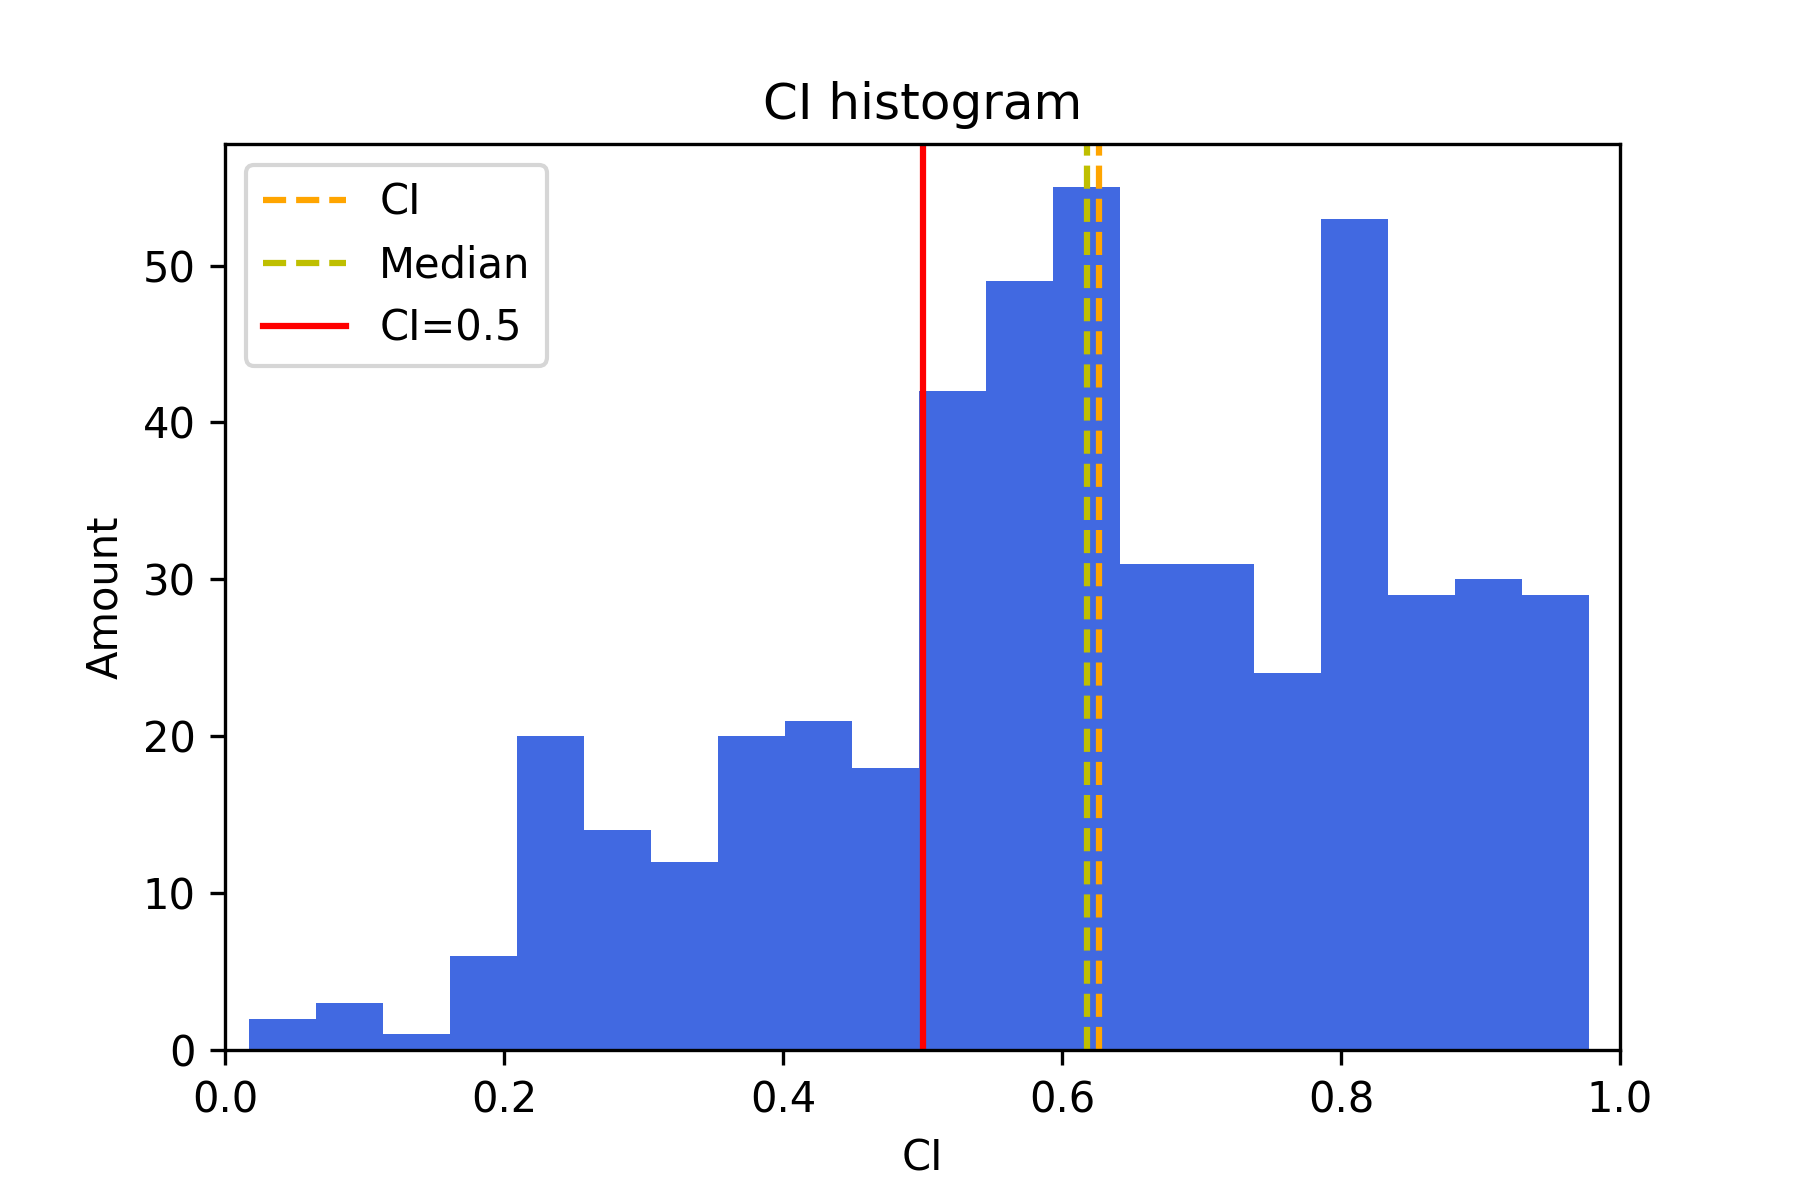
\includegraphics[width=.8\textwidth]{images/results/c-index_volume}
  \caption[LOOCV volume only model results]{
    Volume only model results using \acrshort{LOOCV} \label{fig:results-volume-LOOCV}
    
    Histogram showing the distribution of all the \acrshort{LOOCV} elements' \acrshort{CI}
    when using mixed pairs to obtain the \acrshort{CI}. Final \gls{CI} is 0,627, median
    \gls{CI} is 0,618.
  }
\end{figure}

\ssecc{Build shallow siamese network}
\label{sec:shallow-siamese}

The initial shallow siamese network design had a very simple design for the sister network. 
In fact, it was so simple that a proper \gls{CNN} could not be build, the original design 
can be found in \autoref{fig:shallow-sister}.

The main problem was that there were only two convolutional layers so that when trying to reduce
the image dimension the output image still was too big for a Fully Connected layer. With this
problem in mind a new design was made and it's shown in \autoref{fig:shallow-implement}.

This new design has more layers to reduce the dimensions of the image and is able to 
incorporate the scalar data. As it was previously said this design it's still part of the
siamese network model.

This task took two weeks to complete and no further development will be held with this task
since the next efforts are centered around a model using only the radiomic features.

\begin{figure}
  \centering
  
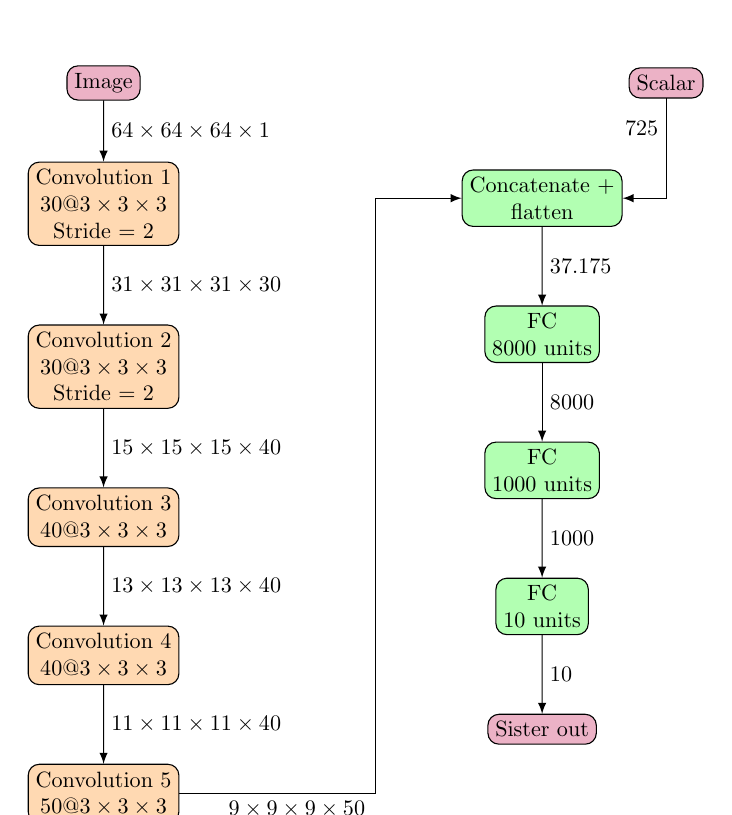
\begin{tikzpicture}[every node/.style={scale=.8}]

  \tikzstyle{module}=[rounded corners, draw, align=center]
  \tikzstyle{FC}=[module, fill=green!30]
  \tikzstyle{conv}=[module, fill=orange!30]
  \tikzstyle{io}=[module, fill=purple!30]
  
  
  \node [io] (image) {Image};
  \node [conv, below = of image] (CNN-1) at (0, 0) {
    Convolution 1 \\ 
    \( 30 @ 3 \times 3 \times 3 \) \\
    Stride = 2
  };
  \node [conv, below = of CNN-1] (CNN-2) {
    Convolution 2 \\
    \( 30 @ 3 \times 3 \times 3 \) \\
    Stride = 2
  };
  \node [conv, below = of CNN-2] (CNN-3) {
    Convolution 3 \\
    \( 40 @ 3 \times 3 \times 3 \)
  };
  \node [conv, below = of CNN-3] (CNN-4) {
    Convolution 4 \\
    \( 40 @ 3 \times 3 \times 3 \)
  };
  \node [conv, below = of CNN-4] (CNN-5) {
    Convolution 5 \\
    \( 50 @ 3 \times 3 \times 3 \)
  };

  \node [right = 5 of image] (aux) {};
  \node [io, right = of aux] (scalar) {Scalar};

  \node [FC, below = of aux] (con) {Concatenate + \\ flatten};
  \node [left = of con] (aux-2) {};
  \node [FC, below = of con] (FC-1) {FC \\ 8000 units};
  \node [FC, below = of FC-1] (FC-2) {FC \\ 1000 units};
  \node [FC, below = of FC-2] (FC-3) {FC \\ 10 units};

  \node [io, below = of FC-3] (out) {Sister out};
  
  \draw [-latex] (image) -- (CNN-1) node[midway, right] {\( 64 \times 64 \times 64 \times 1 \)};
  \draw [-latex] (CNN-1) -- (CNN-2) node[midway, right] {\( 31 \times 31 \times 31 \times 30 \)};
  \draw [-latex] (CNN-2) -- (CNN-3) node[midway, right] {\( 15 \times 15 \times 15 \times 40 \)};
  \draw [-latex] (CNN-3) -- (CNN-4) node[midway, right] {\( 13 \times 13 \times 13 \times 40 \)};
  \draw [-latex] (CNN-4) -- (CNN-5) node[midway, right] {\( 11 \times 11 \times 11 \times 40 \)};

  \draw (CNN-5) -| (aux-2.center)  node[pos=.3, below] {\( 9 \times 9 \times 9 \times 50 \)};
  \draw [-latex] (aux-2.center) |- (con);
  \draw [-latex] (scalar) |- (con) node[pos=.15, left] {\( 725 \)};
  
  \draw [-latex] (con) -- (FC-1) node[midway, right] {\( 37.175 \)};
  \draw [-latex] (FC-1) -- (FC-2) node[midway, right] {\( 8000 \)};
  \draw [-latex] (FC-2) -- (FC-3) node[midway, right] {\( 1000 \)};
  \draw [-latex] (FC-3) -- (out) node[midway, right] {\( 10 \)};
\end{tikzpicture}



  \caption{Shallow siamese sister's network illustration \label{fig:shallow-implement}}
\end{figure}

\sssecc{Results}

The results have been obtained using 4-\gls{CV}. The training parameters where:
\begin{itemize}
  \item Learning rate: 0,001
  \item Regularization factor: 0,01
  \item Number of epochs: 10
  \item Batch size: 40
\end{itemize}
A bigger batch size could not be used because
the model was using a lot of memory. By having a small batch size the number of train 
iterations was of 2.180. The 4-\gls{CV} results can be seen at \autoref{tab:results-shallow-4CV}.

It can be seen that the number of pairs is not the same as in \autoref{tab:results-volume-4CV} 
from the volume model. This is caused by data augmentation. Since
data augmentation is used, there are four images for each patient so the number of pairs
increases too.

The results show a really poor performance, even poorer than random. So, these results
do not improve the current state-of-the-art and are worse than the results that have 
been set to create a baseline. 

It's interesting to highlight that the network has not even learned what it had learned in the 
previous design even being the volume one of the radiomic features
that are passed as input.

\begin{table}
  \centering
  \begin{tabular}{|c||c|c|c||c|c|c|}
    \cline{2-7}
    \multicolumn{1}{c|}{} & \multicolumn{3}{|c||}{\textbf{Pairs}} & 
    \multicolumn{3}{c|}{\textbf{Concordance Index}} \\
    \hline
    \textbf{Fold} & \textbf{Mixed} & \textbf{Train} & \textbf{Test} & 
    \textbf{Mixed} & \textbf{Train} & \textbf{Test} \\
    \hhline{=======}
    0 & 65.436 & 187.216 & 21.320 & 0,43 & 0,42 & 0,419 \\
    1 & 65.436 & 187.828 & 21.112 & 0,444 & 0,431 & 0,459 \\
    2 & 65.392 & 190.308 & 20.336 & 0,472 & 0,474 & 0,426 \\
    3 & 65.392 & 189.096 & 20.704 & 0,514 & 0,512 & 0,514 \\
    \hhline{=======}
    \textbf{Total} & 261.656 & 754.448 & 83.472 & 0,465 & 0,459 & 0,455 \\
    \hline
  \end{tabular}

  \caption[Shallow 4-CV results]{
    Results for shallow model using 4-CV \label{tab:results-shallow-4CV}.
  }
\end{table}

\ssecc{Build scalar only siamese network}
\label{sec:scalar-only}

To speed up the testing process, a siamese network that only used scalar features 
was built. With this approach, the training time was reduced from around 5 hours 
to 1 minute to train a single model. 

To improve the network's performance Dropout \cite{neural:dropout} was used, by using 
dropout some of the model activations are zeroed and then scaled according to the 
dropout probability. This way, the networks' neurons do not have all the information and 
thus they must generalize. Dropout is used as a way of regularization. 

Moreover, since this model inherits from the basic model, defined in \autoref{sec:basic-siamese}, 
regularization is applied too by adding the l2 norm of the weights. The loss and
cost functions are the same too.

To complete this step it took one week but two more weeks were needed to validate the results 
and to fix some bugs.

\begin{figure}
  \centering
  
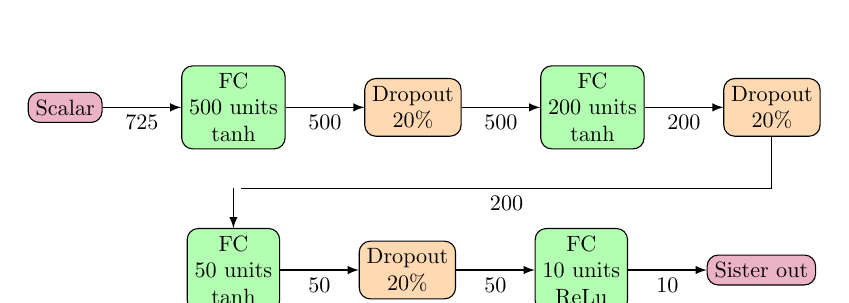
\begin{tikzpicture}[every node/.style={scale=.8}]

  \tikzstyle{module}=[rounded corners, draw, align=center]
  \tikzstyle{FC}=[module, fill=green!30]
  \tikzstyle{conv}=[module, fill=orange!30]
  \tikzstyle{io}=[module, fill=purple!30]

  \node [io] (scalar) {Scalar};

  \node [FC, right = of scalar] (FC-1) {FC \\ 500 units \\ tanh};
  \node [conv, right = of FC-1] (D-1) {Dropout \\ 20\%};
  \node [FC, right = of D-1] (FC-2) {FC \\ 200 units \\ tanh};
  \node [conv, right = of FC-2] (D-2) {Dropout \\ 20\%};

  \node [FC, below = of FC-1] (FC-3) {FC \\ 50 units \\ tanh};
  \node [conv, right = of FC-3] (D-3) {Dropout \\ 20\%};
  \node (aux) at ($(FC-3)!0.5!(FC-1)$) {};
  \node [FC, right = of D-3] (FC-4) {FC \\ 10 units \\ ReLu};


  \node [io, right = of FC-4] (out) {Sister out};
  \draw [-latex] (scalar) -- (FC-1) node[midway, below] {\( 725 \)};

  \draw [-latex] (FC-1) -- (D-1) node[midway, below] {\( 500 \)};
  \draw [-latex] (D-1) -- (FC-2) node[midway, below] {\( 500 \)};
  \draw [-latex] (FC-2) -- (D-2) node[midway, below] {\( 200 \)};
  
  \draw [-latex] (D-2) |- node[pos=.75, below]{\( 200 \)} (aux) -| (FC-3);
  \draw [-latex] (FC-3) -- (D-3) node[midway, below] {\( 50 \)};
  \draw [-latex] (D-3) -- (FC-4) node[midway, below] {\( 50 \)};
  \draw [-latex] (FC-4) -- (out) node[midway, below] {\( 10 \)};

  % \draw [-latex] (FC-3) -- (out) node[midway, below] {\( 10 \)};
\end{tikzpicture}



  \caption{Scalar siamese network illustration \label{fig:scalar-implement}}
\end{figure}

\sssecc{Results}

The results obtained with this model are both with 4-CV and \gls{LOOCV}. The training 
parameters have been the following ones:
\begin{itemize}
  \item Learning rate: 0,001
  \item Regularization factor: 0,01
  \item Dropout probability: 0,2/1
  \item Number of epochs: 1000
  \item Batch size: The whole dataset
\end{itemize}

A summary of the results using 4-CV can be seen at \autoref{tab:results-scalar-4CV}. It can be
observed that the number of pairs is not constant through all the folds. This is caused by
censoring, since not all members can form a pair with all the other ones some elements 
have more available pairs than others. 

From the 4-CV results it can be seen that the final test \gls{CI} is 0,635 and the final mixed 
\gls{CI} is 0,764. Even thought it seems that the test results are very similar to the
state-of-the art (0,628) when compared to the baseline the test results are similar but
the mixed pairs results have improved (0,764 vs 0,616).

The improvement with the baseline is relevant because the final objective of the project
is to create a model to predict a patient's survival time. The final method to predict
survival will be to compare a new patient against the whole training set and then, having
all the comparisons and the survival time of the train set's patients, a prediction of
the new patient's survival time can will be made. This means that the most relevant 
indicator is the mixed \gls{CI}.

The results using \gls{LOOCV} can be seen represented in \autoref{fig:results-scalar-LOOCV}. 
In this case, only the mixed pairs have been compared to create the histogram.

The final \gls{CI} with \gls{LOOCV} is 0,771 while the median \gls{CI} is 0,862. The final 
\gls{CI} using \gls{LOOCV} is very similar to the one obtained using 4-CV (0,771 vs 0,764).

\begin{table}
  \centering
  \begin{tabular}{|c||c|c|c||c|c|c|}
    \cline{2-7}
    \multicolumn{1}{c|}{} & \multicolumn{3}{|c||}{\textbf{Pairs}} & 
    \multicolumn{3}{c|}{\textbf{Concordance Index}} \\
    \hline
    \textbf{Fold} & \textbf{Mixed} & \textbf{Train} & \textbf{Test} & 
    \textbf{Mixed} & \textbf{Train} & \textbf{Test} \\
    \hhline{=======}
    0 & 16.359 & 46.804 & 5.330 & 0,728 & 0,915 & 0,543 \\
    1 & 16.359 & 46.957 & 5.278 & 0,809 & 0,927 & 0,64 \\
    2 & 16.348 & 47.577 & 5.084 & 0,751 & 0,91 & 0,675 \\
    3 & 16.348 & 47.274 & 5.176 & 0,766 & 0,919 & 0,624 \\
    \hhline{=======}
    \textbf{Total} & 65.414 & 188.612 & 20.868 & 0,764 & 0,918 & 0,62   \\
    \hline
  \end{tabular}

  \caption[Scalar Only 4-CV results]{
    Results for scalar only model using 4-CV \label{tab:results-scalar-4CV}
  }
\end{table}

\begin{figure}
  \centering
  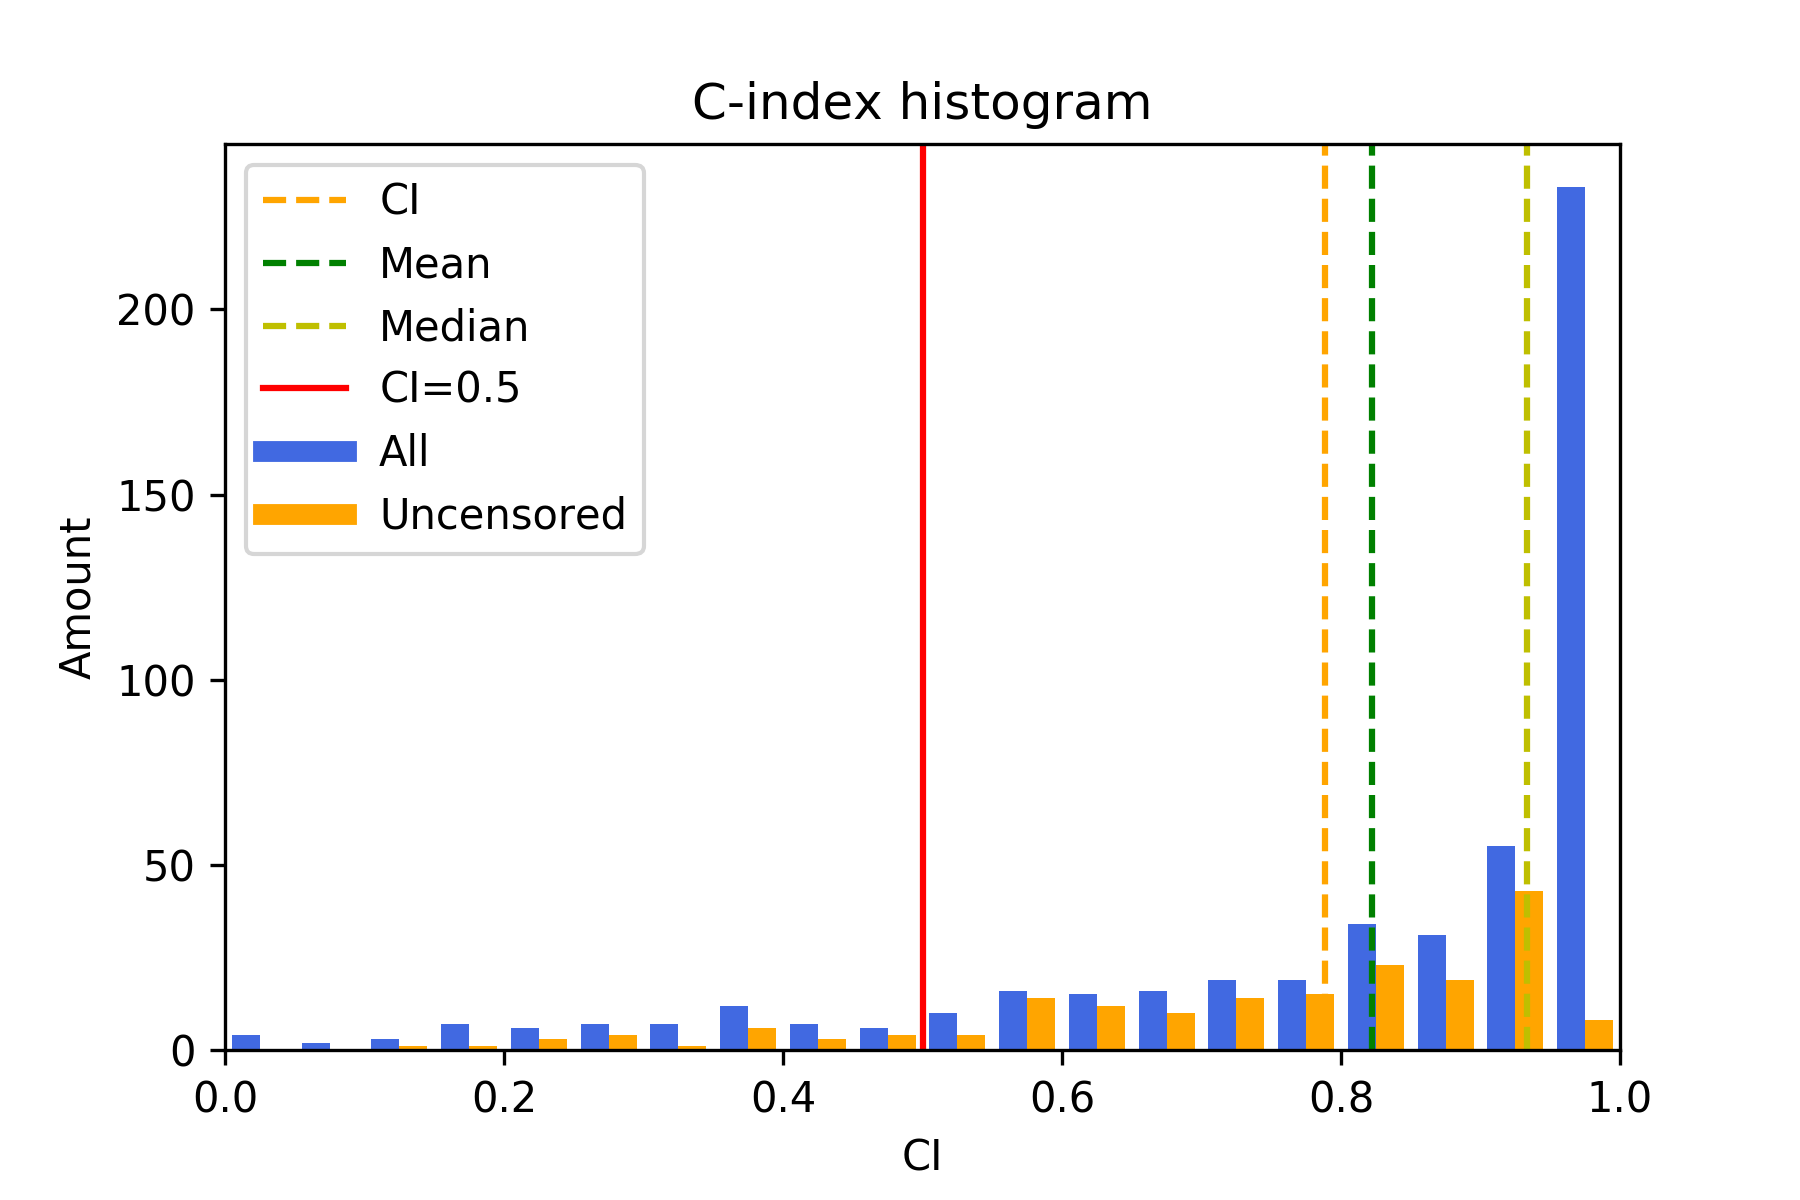
\includegraphics[width=.8\textwidth]{images/results/c-index_scalar}
  \caption[LOOCV scalar only model results]{
    Scalar only model results using \acrshort{LOOCV} \label{fig:results-scalar-LOOCV}
    
    Histogram showing the distribution of all the \acrshort{LOOCV} elements' \acrshort{CI}
    when using mixed pairs to obtain the \acrshort{CI}. Final \gls{CI} is 0,771, median 
    \gls{CI} is 0,862.
  }
\end{figure}

\ssecc{Build deep siamese network}

The deep siamese network design is derived by the Shallow Siamese design shown in 
\autoref{sec:shallow-siamese} although it has more convolutional layers and defines 
multiple types of blocks that are used through the network. As the previous design,
it uses both the radiomic scalar features and the images extracted from the \gls{CT} 
scans. 

Moreover, the design is also inspired in Inception-ResNet-v1 which in turn is 
inspired in Inception-v4 \cite{neural:inception-4}. The whole network's structure can be 
seen in \autoref{fig:residual-general}.

The network is composed by a total of seven convolutional blocks, a final
pooling layer and three more fully connected layers where the radiomic scalar features are
injected. Only the Stem (\autoref{fig:residual-block-stem}), 
Reduction A (\autoref{fig:residual-block-reduce-a}) and
Reduction B (\autoref{fig:residual-block-reduce-b}) blocks reduce the image dimensions,
while the A (\autoref{fig:residual-block-a}) and B (\autoref{fig:residual-block-b}) 
blocks are useful to learn deep features.

\begin{figure}
  \centering
  
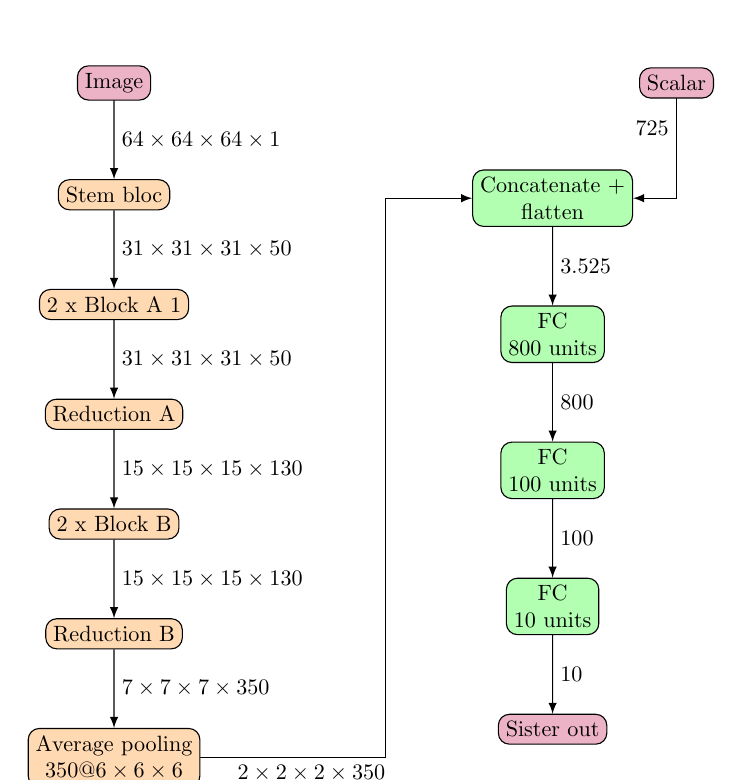
\begin{tikzpicture}[every node/.style={scale=.8}]

  \tikzstyle{module}=[rounded corners, draw, align=center]
  \tikzstyle{FC}=[module, fill=green!30]
  \tikzstyle{conv}=[module, fill=orange!30]
  \tikzstyle{io}=[module, fill=purple!30]
  
  
  \node [io] (image) {Image};

  \node [conv, below = of image] (S) {Stem bloc};
  \node [conv, below = of S] (BA) {2 x Block A 1};
  \node [conv, below = of BA] (R-A) {Reduction A};
  \node [conv, below = of R-A] (BB) {2 x Block B};
  \node [conv, below = of BB] (R-B) {Reduction B};
  \node [conv, below = of R-B] (P) {
    Average pooling \\
    \( 350 @ 6 \times 6 \times 6 \)
  };

  \node [right = 5 of image] (aux) {};
  \node [io, right = of aux] (scalar) {Scalar};

  \node [FC, below = of aux] (con) {Concatenate + \\ flatten};
  \node [left = of con] (aux-2) {};
  \node [FC, below = of con] (FC-1) {FC \\ 800 units};
  \node [FC, below = of FC-1] (FC-2) {FC \\ 100 units};
  \node [FC, below = of FC-2] (FC-3) {FC \\ 10 units};

  \node [io, below = of FC-3] (out) {Sister out};

  \draw [-latex] (image) -- (S) node[midway, right] {\( 64 \times 64 \times 64 \times 1 \)};
  \draw [-latex] (S) -- (BA) node[midway, right] {\( 31 \times 31 \times 31 \times 50 \)};
  \draw [-latex] (BA) -- (R-A) node[midway, right] {\( 31 \times 31 \times 31 \times 50 \)};
  \draw [-latex] (R-A) -- (BB) node[midway, right] {\( 15 \times 15 \times 15 \times 130 \)};
  \draw [-latex] (BB) -- (R-B) node[midway, right] {\( 15 \times 15 \times 15 \times 130 \)};
  \draw [-latex] (R-B) -- (P) node[midway, right] {\( 7 \times 7 \times 7 \times 350 \)};

  \draw (P) -| (aux-2.center)  node[pos=.3, below] {\( 2 \times 2 \times 2 \times 350 \)};
  \draw [-latex] (aux-2.center) |- (con);
  \draw [-latex] (scalar) |- (con) node[pos=.15, left] {\( 725 \)};
  
  \draw [-latex] (con) -- (FC-1) node[midway, right] {\( 3.525 \)};
  \draw [-latex] (FC-1) -- (FC-2) node[midway, right] {\( 800 \)};
  \draw [-latex] (FC-2) -- (FC-3) node[midway, right] {\( 100 \)};
  \draw [-latex] (FC-3) -- (out) node[midway, right] {\( 10 \)};
\end{tikzpicture}



  \caption[Deep siamese network main structure]{
    Deep siamese network main structure \label{fig:residual-general}
    
    The drawing represents the design used for the sister network in the deep siamese
    network design.
  }
\end{figure}
\begin{figure}
  \centering
  \begin{subfigure}[b]{.4\textwidth}
    \centering
    \scalebox{.9}{
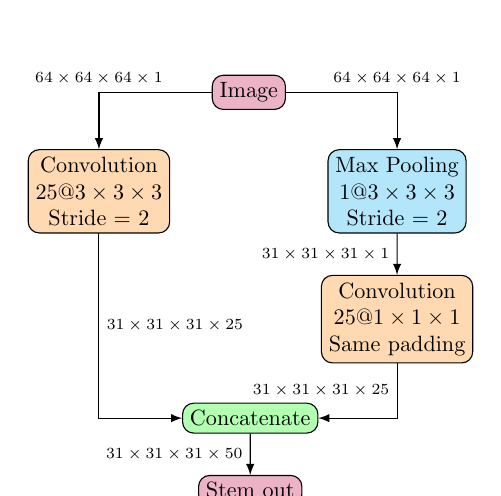
\begin{tikzpicture}[every node/.style={scale=.8}, node distance = 1.5 em]

  \tikzstyle{module}=[rounded corners, draw, align=center]
  \tikzstyle{FC}=[module, fill=green!30]
  \tikzstyle{conv}=[module, fill=orange!30]
  \tikzstyle{pool}=[module, fill=cyan!30]
  \tikzstyle{io}=[module, fill=purple!30]
  \tikzstyle{tensor}=[font=\scriptsize\selectfont]
  
  
  \node [io] (image) {Image};

  \node [conv, below left = 0.5 and 1 of image.south] (A) {
    Convolution \\
    \( 25 @ 3 \times 3 \times 3 \) \\
    Stride = 2
  };
  \node [pool, below right = 0.5 and 1 of image.south] (B-0) {
    Max  Pooling \\
    \( 1 @ 3 \times 3 \times 3 \) \\
    Stride = 2
  };
  \node [conv, below = of B-0] (B-1) {
    Convolution \\
    \( 25 @ 1 \times 1 \times 1 \) \\
    Same padding
  };

  \node [FC, below left = .5 and 1 of B-1.south] (con) {Concatenate};
  \node [io, below = of con] (out) {Stem out};

  \draw [-latex] (image) -| (A) node[tensor, midway, above] {\( 64 \times 64 \times 64 \times 1 \)};
  \draw [-latex] (image) -| (B-0) node[tensor, midway, above] {\( 64 \times 64 \times 64 \times 1 \)};
  \draw [-latex] (B-0) -- (B-1) node[tensor, midway, left] {\( 31 \times 31 \times 31 \times 1 \)};
  \draw [-latex] (B-1) |- (con) node[tensor, near start, left] {\( 31 \times 31 \times 31 \times 25 \)};
  \draw [-latex] (A) |- (con) node[tensor, near start, right] {\( 31 \times 31 \times 31 \times 25 \)};
  \draw [-latex] (con) -- (out) node[tensor, midway, left] {\( 31 \times 31 \times 31 \times 50 \)};

\end{tikzpicture}


}
    \caption{Residual network Stem Block \label{fig:residual-block-stem}}
  \end{subfigure}
  \hfill
  \begin{subfigure}[b]{.59\textwidth}
    \centering
    \scalebox{.9}{
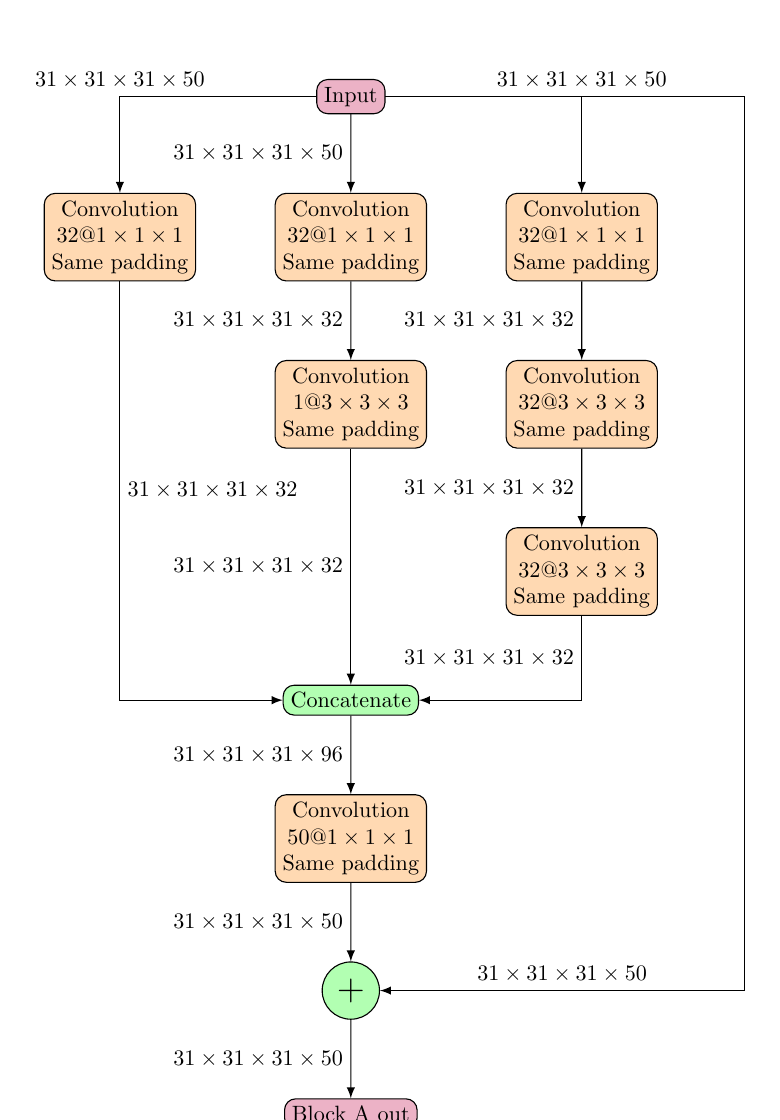
\begin{tikzpicture}[every node/.style={scale=.8}]

  \tikzstyle{module}=[rounded corners, draw, align=center]
  \tikzstyle{FC}=[module, fill=green!30]
  \tikzstyle{conv}=[module, fill=orange!30]
  \tikzstyle{io}=[module, fill=purple!30]
  
  
  \node [io] (image) {Input};

  \node [conv, below = of image] (B-C-0) {
    Convolution \\
    \( 32 @ 1 \times 1 \times 1 \) \\
    Same padding
  };
  \node [conv, below = of B-C-0] (B-C-1) {
    Convolution \\
    \( 1 @ 3 \times 3 \times 3 \) \\
    Same padding
  };

  \node [conv, left = of B-C-0] (A-C) {
    Convolution \\
    \( 32 @ 1 \times 1 \times 1 \) \\
    Same padding
  };
  \node [conv, right = of B-C-0] (C-C-0) {
    Convolution \\
    \( 32 @ 1 \times 1 \times 1 \) \\
    Same padding
  };
  \foreach \x [remember=\x as \lastx (initially 0)] in {1,2} {
    \node [conv, below = of C-C-\lastx] (C-C-\x) {
      Convolution \\
      \( 32 @ 3 \times 3 \times 3 \) \\
      Same padding
    };
  }

  \node [FC, below = 3 of B-C-1] (con) {Concatenate};
  
  \node [conv, below = of con] (F-C) {
    Convolution \\
    \( 50 @ 1 \times 1 \times 1 \) \\
    Same padding
    };
  \node [circle, FC, below = of F-C] (sum) {\LARGE +};
  \node [io, below = of sum] (out) {Block A out};

  \node [right = of C-C-0] (aux) {};

  \draw [-latex] (image) -| (A-C) node[midway, above] {\( 31 \times 31 \times 31 \times 50 \)};
  \draw [-latex] (image) -- (B-C-0) node[midway, left] {\( 31 \times 31 \times 31 \times 50 \)};
  \draw [-latex] (image) -| (C-C-0) node[midway, above] {\( 31 \times 31 \times 31 \times 50 \)};

  \draw [-latex] (B-C-0) -- (B-C-1) node[midway, left] {\( 31 \times 31 \times 31 \times 32 \)};
  \draw [-latex] (C-C-0) -- (C-C-1) node[midway, left] {\( 31 \times 31 \times 31 \times 32 \)};
  \draw [-latex] (C-C-1) -- (C-C-2) node[midway, left] {\( 31 \times 31 \times 31 \times 32 \)};

  \draw [-latex] (A-C) |- (con) node[near start, right] {\( 31 \times 31 \times 31 \times 32 \)};
  \draw [-latex] (B-C-1) -- (con) node[midway, left] {\( 31 \times 31 \times 31 \times 32 \)};
  \draw [-latex] (C-C-2) |- (con) node[near start, left] {\( 31 \times 31 \times 31 \times 32 \)};

  \draw [-latex] (con) -- (F-C) node[midway, left] {\( 31 \times 31 \times 31 \times 96 \)};
  \draw [-latex] (F-C) -- (sum) node[midway, left] {\( 31 \times 31 \times 31 \times 50 \)};
  \draw (image) -| (aux.center);
  \draw [-latex] (aux.center) |- (sum) node[near end, above] {\( 31 \times 31 \times 31 \times 50 \)};
  \draw [-latex] (sum) -- (out) node[midway, left] {\( 31 \times 31 \times 31 \times 50 \)};

\end{tikzpicture}


}
    \caption{Residual network convolutional Block A \label{fig:residual-block-a}}
  \end{subfigure}
  \caption{Residual Network blocks}
\end{figure}

\begin{figure}\ContinuedFloat
  \begin{subfigure}[b]{.49\textwidth}
    \centering
    \scalebox{.9}{
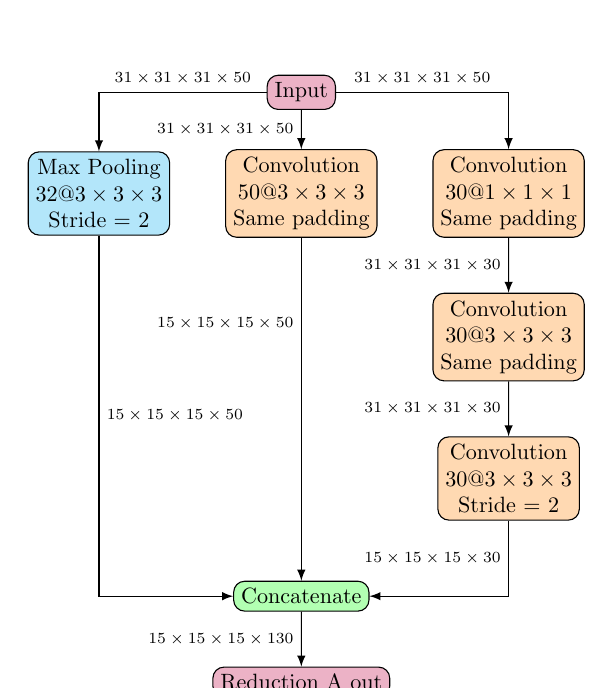
\begin{tikzpicture}[every node/.style={scale=.8}, node distance = 0.7]

  \tikzstyle{module}=[rounded corners, draw, align=center]
  \tikzstyle{FC}=[module, fill=green!30]
  \tikzstyle{conv}=[module, fill=orange!30]
  \tikzstyle{pool}=[module, fill=cyan!30]
  \tikzstyle{io}=[module, fill=purple!30]
  \tikzstyle{tensor}=[font=\scriptsize\selectfont]
  
  
  \node [io] (image) {Input};

  \node [conv, below = 0.5 and 1 of image] (B-0) {
    Convolution \\
    \( 50 @ 3  \times 3 \times 3 \) \\
    Same padding
  };

  \node [pool, left = of B-0] (A) {
    Max Pooling \\
    \( 32 @ 3 \times 3 \times 3 \) \\
    Stride = 2
  };
  \node [conv, right = of B-0] (C-0) {
    Convolution \\
    \( 30 @ 1 \times 1 \times 1 \) \\
    Same padding
  };
  \node [conv, below = of C-0] (C-1) {
    Convolution \\
    \( 30 @ 3 \times 3 \times 3 \) \\
    Same padding
  };
  \node [conv, below = of C-1] (C-2) {
    Convolution \\
    \( 30 @ 3 \times 3 \times 3 \) \\
    Stride = 2
  };

  \node (aux-1) at ($(C-2 -| B-0) + (0, -.5)$) {};

  \node [FC, below = of aux-1] (con) {Concatenate};
  \node [io, below = of con] (out) {Reduction A out};

  \draw [-latex] (image) -| (A) node[tensor, near start, above] {\( 31 \times 31 \times 31 \times 50 \)};
  \draw [-latex] (image) -- (B-0) node[tensor, midway, left] {\( 31 \times 31 \times 31 \times 50 \)};
  \draw [-latex] (image) -| (C-0) node[tensor, near start, above] {\( 31 \times 31 \times 31 \times 50 \)};

  \draw [-latex] (C-0) -- (C-1) node[tensor, midway, left] {\( 31 \times 31 \times 31 \times 30 \)};
  \draw [-latex] (C-1) -- (C-2) node[tensor, midway, left] {\( 31 \times 31 \times 31 \times 30 \)};

  \draw [-latex] (A) |- (con) node[tensor, near start, right] {\( 15 \times 15 \times 15 \times 50 \)};
  \draw [-latex] (B-0) -- (con) node[tensor, near start, left] {\( 15 \times 15 \times 15 \times 50 \)};
  \draw [-latex] (C-2) |- (con) node[tensor, near start, left] {\( 15 \times 15 \times 15 \times 30 \)};

  \draw [-latex] (con) -- (out) node[tensor, midway, left] {\( 15 \times 15 \times 15 \times 130 \)};

\end{tikzpicture}


}
    \caption{Residual network Reduction A \label{fig:residual-block-reduce-a}}
  \end{subfigure}
  \begin{subfigure}[b]{.49\textwidth}
    \centering
    \scalebox{.9}{
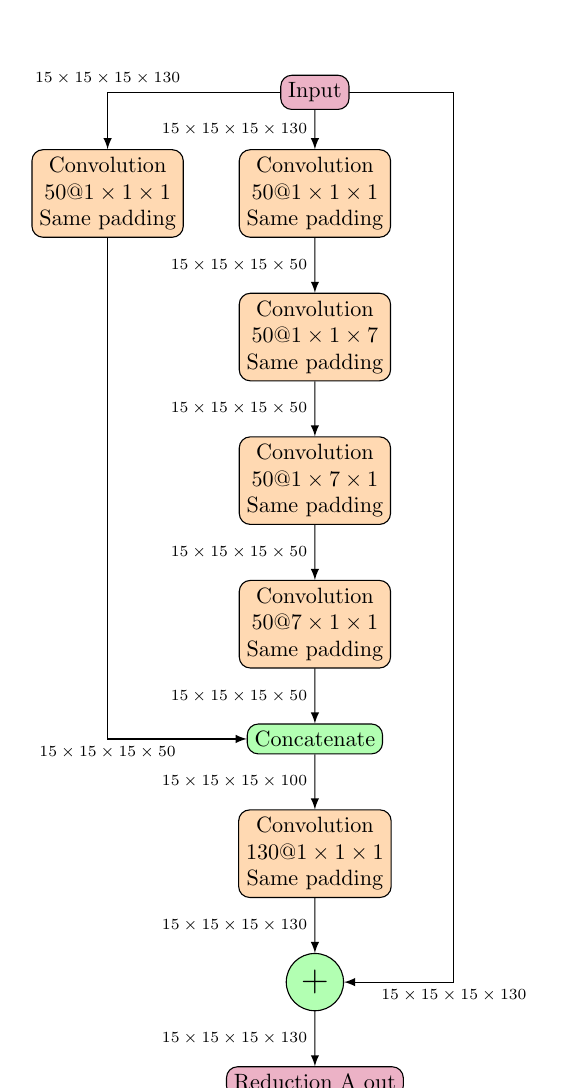
\begin{tikzpicture}[every node/.style={scale=.8}, node distance = 0.7]

  \tikzstyle{module}=[rounded corners, draw, align=center]
  \tikzstyle{FC}=[module, fill=green!30]
  \tikzstyle{conv}=[module, fill=orange!30]
  \tikzstyle{pool}=[module, fill=cyan!30]
  \tikzstyle{io}=[module, fill=purple!30]
  \tikzstyle{tensor}=[font=\scriptsize\selectfont]
  
  
  \node [io] (image) {Input};

  \node [conv, below = 0.5 of image] (B-C-0) {
    Convolution \\
    \( 50 @ 1 \times 1 \times 1 \) \\
    Same padding
  };
  \node [conv, below = of B-C-0] (B-C-1) {
    Convolution \\
    \( 50 @ 1  \times 1 \times 7 \) \\
    Same padding
  };
  \node [conv, below = of B-C-1] (B-C-2) {
    Convolution \\
    \( 50 @ 1  \times 7 \times 1 \) \\
    Same padding
  };
  \node [conv, below = of B-C-2] (B-C-3) {
    Convolution \\
    \( 50 @ 7  \times 1 \times 1 \) \\
    Same padding
  };

  \node [conv, left = of B-C-0] (A-C) {
    Convolution \\
    \( 50 @ 1 \times 1 \times 1 \) \\
    Same padding
  };

  \node [right = of B-C-0] (aux-1) {};

  \node [FC, below = of B-C-3] (con) {Concatenate};

  \node [conv, below = of con] (F-C) {
    Convolution \\
    \( 130 @ 1 \times 1 \times 1 \) \\
    Same padding
    };
  \node [circle, FC, below = of F-C] (sum) {\LARGE +};

  \node [io, below = of sum] (out) {Reduction A out};

  \draw [-latex] (image) -| (A-C) node[tensor, midway, above] {\( 15 \times 15 \times 15 \times 130 \)};
  \draw [-latex] (image) -- (B-C-0) node[tensor, midway, left] {\( 15 \times 15 \times 15 \times 130 \)};
  
  \draw [-latex] (A-C) |- (con) node[tensor, midway, below] {\( 15 \times 15 \times 15 \times 50 \)};
  \draw [-latex] (B-C-0) -- (B-C-1) node[tensor, midway, left] {\( 15 \times 15 \times 15 \times 50 \)};
  \draw [-latex] (B-C-1) -- (B-C-2) node[tensor, midway, left] {\( 15 \times 15 \times 15 \times 50 \)};
  \draw [-latex] (B-C-2) -- (B-C-3) node[tensor, midway, left] {\( 15 \times 15 \times 15 \times 50 \)};
  \draw [-latex] (B-C-3) -- (con) node[tensor, midway, left] {\( 15 \times 15 \times 15 \times 50 \)};
  
  \draw (image) -| (aux-1.center);
  \draw [-latex] (aux-1.center) |- (sum) node[tensor, midway, below] {\( 15 \times 15 \times 15 \times 130 \)};
  
  \draw [-latex] (F-C) -- (sum) node[tensor, midway, left] {\( 15 \times 15 \times 15 \times 130 \)};
  \draw [-latex] (con) -- (F-C) node[tensor, midway, left] {\( 15 \times 15 \times 15 \times 100 \)};
  \draw [-latex] (sum) -- (out) node[tensor, midway, left] {\( 15 \times 15 \times 15 \times 130 \)};

\end{tikzpicture}


}
    \caption{Residual network Block B \label{fig:residual-block-b}}
  \end{subfigure}

  \begin{subfigure}[b]{\textwidth}
    \centering
    \scalebox{.9}{
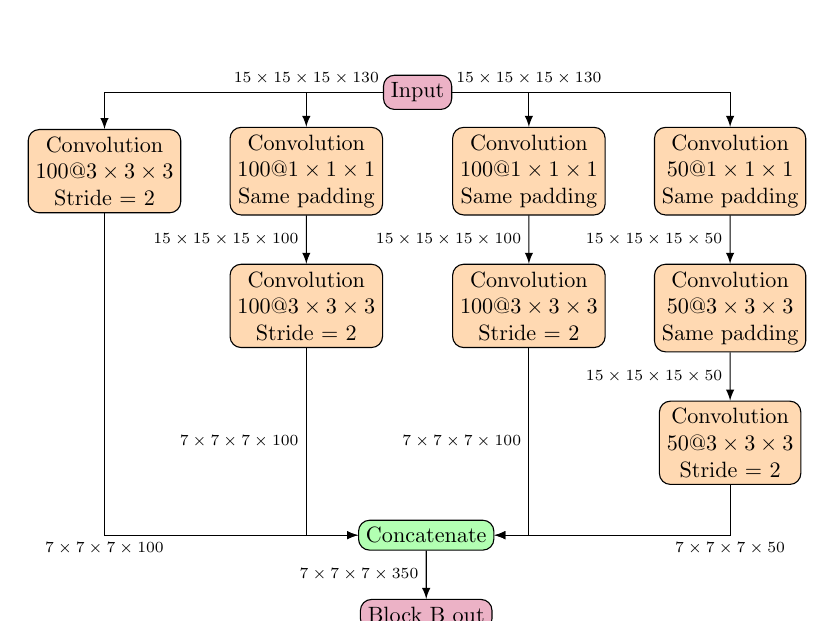
\begin{tikzpicture}[every node/.style={scale=.8}, node distance = 0.7, x=2.5em, y=2.5em]

  \tikzstyle{module}=[rounded corners, draw, align=center,]
  \tikzstyle{FC}=[module, fill=green!30]
  \tikzstyle{conv}=[module, fill=orange!30]
  \tikzstyle{pool}=[module, fill=cyan!30]
  \tikzstyle{io}=[module, fill=purple!30]
  \tikzstyle{tensor}=[font=\scriptsize\selectfont]
  
  
  \node [io] (image) {Input};

  \node [conv, below left = .5 and .5 of image.center] (B-0) {
    Convolution \\
    \( 100 @ 1 \times 1 \times 1 \) \\
    Same padding
  };
  \node [conv, below = of B-0] (B-1) {
    Convolution \\
    \( 100 @ 3 \times 3 \times 3 \) \\
    Stride = 2
  };

  \node [conv, left = of B-0] (A) {
    Convolution \\
    \( 100 @ 3 \times 3 \times 3 \) \\
    Stride = 2
  };

  \node [conv, below right = .5 and .5 of image.center] (C-0) {
    Convolution \\
    \( 100 @ 1 \times 1 \times 1 \) \\
    Same padding
  };

  \node [conv, below = of C-0] (C-1) {
    Convolution \\
    \( 100 @ 3 \times 3 \times 3 \) \\
    Stride = 2
  };

  \node [conv, right = of C-0] (D-0) {
    Convolution \\
    \( 50 @ 1 \times 1 \times 1 \) \\
    Same padding
  };

  \node [conv, below = of D-0] (D-1) {
    Convolution \\
    \( 50 @ 3 \times 3 \times 3 \) \\
    Same padding
  };

  \node [conv, below = of D-1] (D-2) {
    Convolution \\
    \( 50 @ 3 \times 3 \times 3 \) \\
    Stride = 2
  };

  \node (aux-1) at ($(D-2 -| C-1) + (0, -.5)$) {};

  \node [FC, below left = .5 and .5 of aux-1.south] (con) {Concatenate};
  \node [io, below = of con] (out) {Block B out};

  \draw [-latex] (image) -| (A);
  \draw [-latex] (image) -| (B-0) node[tensor, midway, above] {\( 15 \times 15 \times 15 \times 130 \)};
  \draw [-latex] (image) -| (C-0) node[tensor, midway, above] {\( 15 \times 15 \times 15 \times 130 \)};
  \draw [-latex] (image) -| (D-0);
  
  \draw [-latex] (A) |- (con) node[tensor, midway, below] {\( 7 \times 7 \times 7 \times 100 \)};

  \draw [-latex] (B-0) -- (B-1) node[tensor, midway, left] {\( 15 \times 15 \times 15 \times 100 \)};
  \draw [-latex] (B-1) |- (con) node[tensor, near start, left] {\( 7 \times 7 \times 7 \times 100 \)};
  
  \draw [-latex] (C-0) -- (C-1) node[tensor, midway, left] {\( 15 \times 15 \times 15 \times 100 \)};
  \draw [-latex] (C-1) |- (con) node[tensor, near start, left] {\( 7 \times 7 \times 7 \times 100 \)};
  
  \draw [-latex] (D-0) -- (D-1) node[tensor, midway, left] {\( 15 \times 15 \times 15 \times 50 \)};
  \draw [-latex] (D-1) -- (D-2) node[tensor, midway, left] {\( 15 \times 15 \times 15 \times 50 \)};
  \draw [-latex] (D-2) |- (con) node[tensor, midway, below] {\( 7 \times 7 \times 7 \times 50 \)};

  \draw [-latex] (con) -- (out) node[tensor, midway, left] {\( 7 \times 7 \times 7 \times 350 \)};

\end{tikzpicture}


}
    \caption{Residual network Block B \label{fig:residual-block-reduce-b}}
  \end{subfigure}
  \caption{Residual Network blocks (continuation)}
\end{figure}

\sssecc{Results}

To get the results for the deep siamese network 4-\gls{CV} has been used. The training
parameters are the following ones:
\begin{itemize}
  \item Learning rate: 0,001
  \item Regularization factor: 0,01
  \item Dropout probability: 0,2/1
  \item Number of epochs: 15
  \item Batch size: 20
\end{itemize}

The results with this training can be seen in \autoref{tab:results-residual-4CV}, the final
mixed \gls{CI} is 0,601 while the final train \gls{CI} is 0,603.
As it can be seen in \autoref{fig:results-residual-CI} only two of the four folds have 
properly converged to a solution when training the residual model, while the other two folds
have stayed in a random \gls{CI}. The two folds that have properly converged have been able
to obtain an average mixed \gls{CI} of 0,793 which is similar to the results using only
the scalar radiomic features (0,793 vs 0,771).

Future work on this task will be to find the proper hyper-parameters to make sure that all
the folds can finally converge and then train the model using \gls{LOOCV} to make sure
that not only certain distributions are able to show this behavior.

\begin{table}
  \centering
  \begin{tabular}{|c||c|c|c||c|c|c|}
    \cline{2-7}
    \multicolumn{1}{c|}{} & \multicolumn{3}{|c||}{\textbf{Pairs}} & 
    \multicolumn{3}{c|}{\textbf{Concordance Index}} \\
    \hline
    \textbf{Fold} & \textbf{Mixed} & \textbf{Train} & \textbf{Test} & 
    \textbf{Mixed} & \textbf{Train} & \textbf{Test} \\
    \hhline{=======}
    0 & 65.436 & 187.216 & 21.320 & 0,765 & 0,812 & 0,814 \\
    1 & 65.436 & 187.828 & 21.112 & 0,821 & 0,813 & 0,813 \\
    2 & 65.392 & 190.308 & 20.336 & 0,427 & 0,431 & 0,387 \\
    3 & 65.392 & 189.096 & 20.704 & 0,389 & 0,359 & 0,428 \\
    \hhline{=======}
    \textbf{Total} & 261.656 & 754.448 & 83.472 & 0,601 & 0,603 & 0,614 \\
    \hline
  \end{tabular}

  \caption[Residual 4-CV results]{
    Results for residual model using 4-CV \label{tab:results-residual-4CV}
  }
\end{table}

\begin{figure}
  \centering
  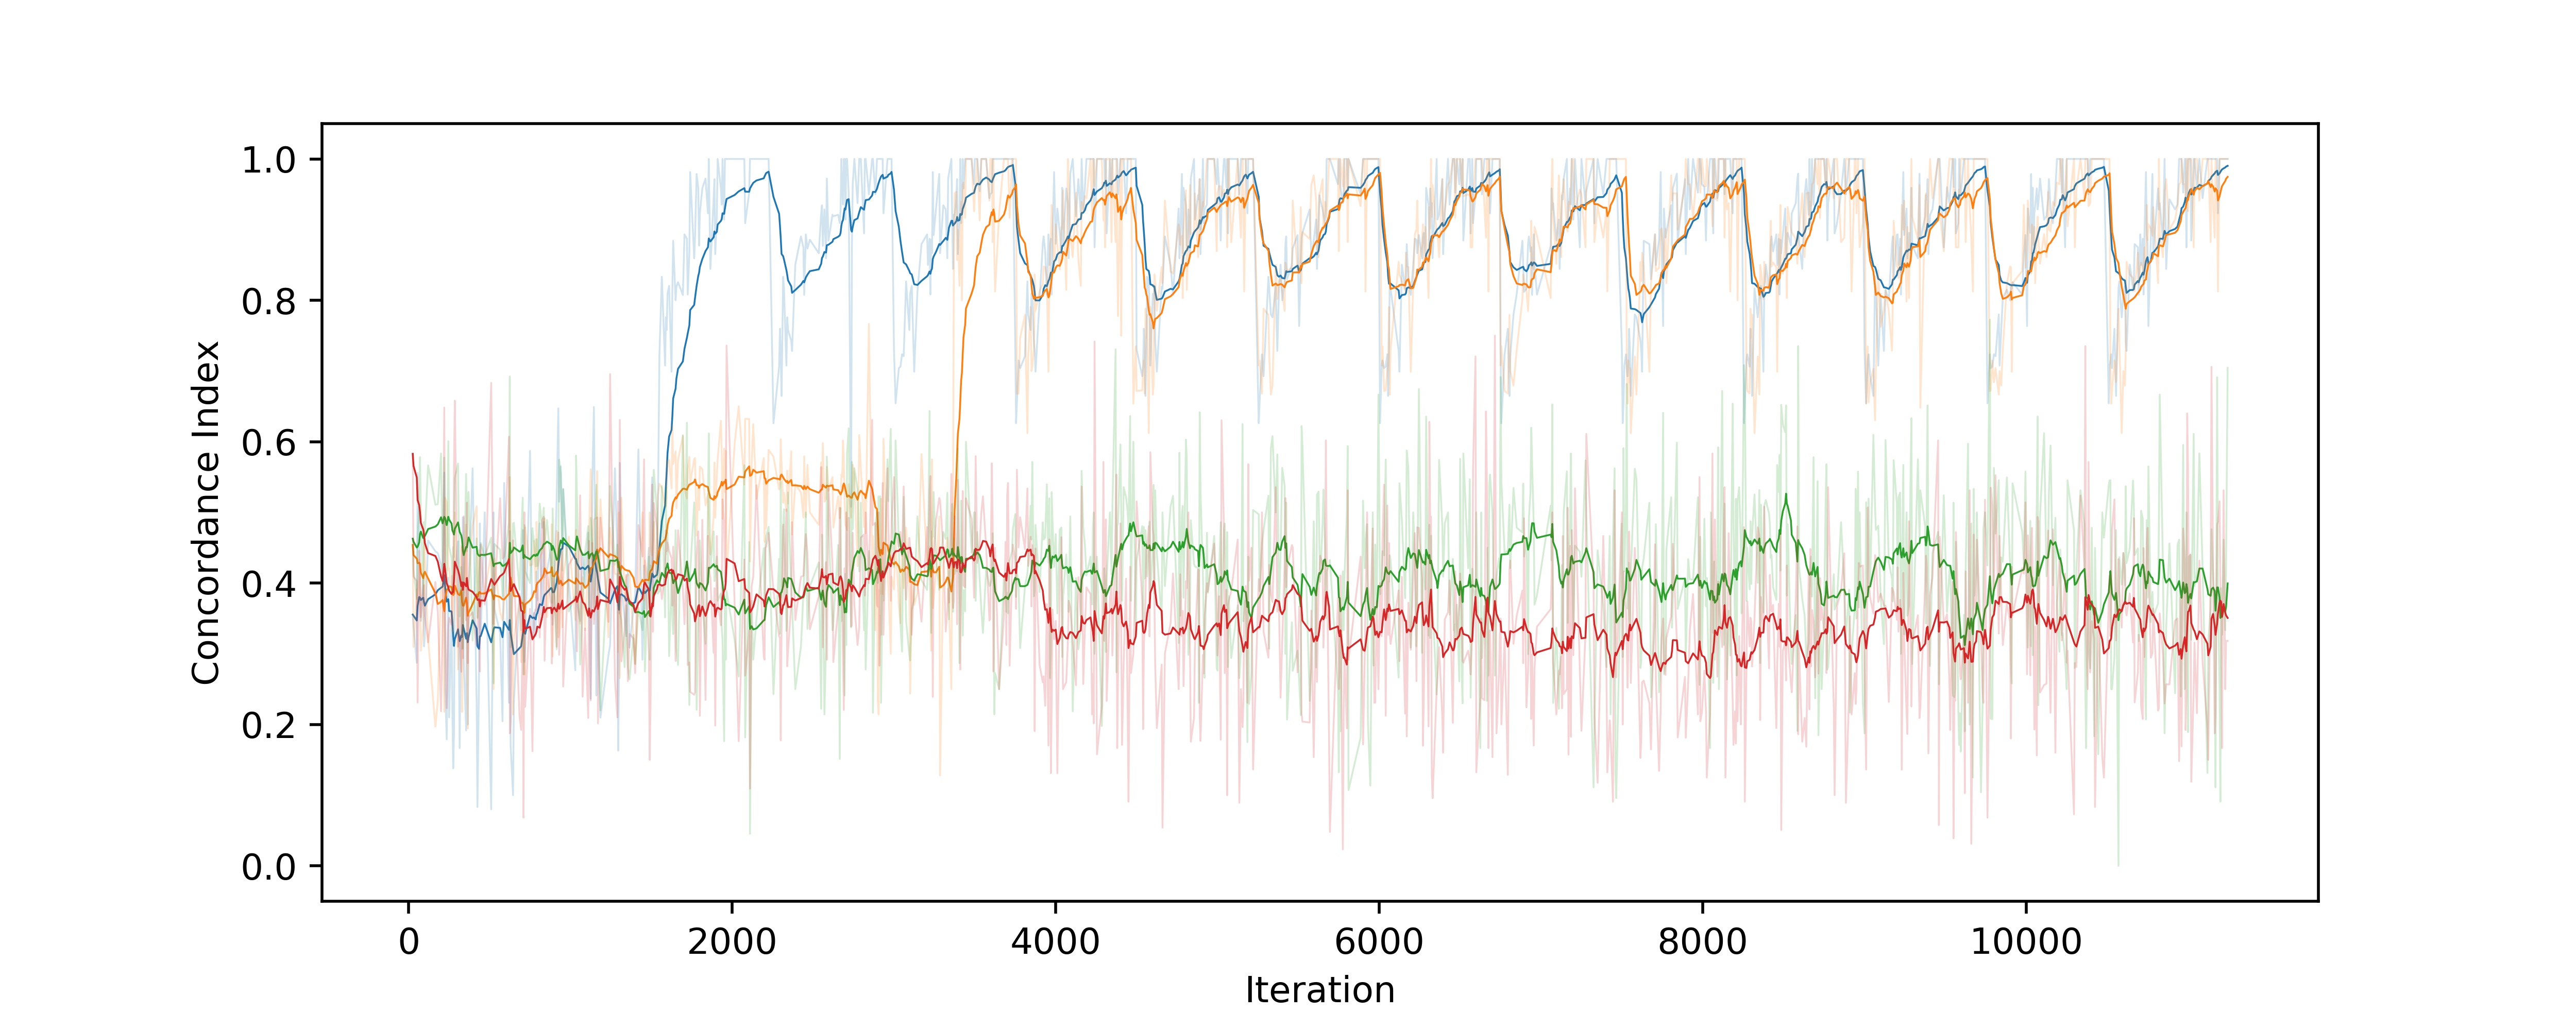
\includegraphics[width=\textwidth]{images/results/residual_train}

  \caption[Training iterations \gls{CI}]{
    \gls{CI} during training iterations for each one of the 4-\gls{CV} folds. Each 
    color represents a different fold. The real data is shown in a lighter color, as some
    smoothing has been applied to show the tendency.

    \label{fig:results-residual-CI}
  }
\end{figure}

\ssecc{Predict patients survival}

Once one of the siamese models is working the next step is to predict a patient's survival
time. A basic approach would be to predict if they will be a long or short survival time 
patient. Multiple ideas have been brainstormed although not all of them have been tested.

The difficulty of the problem resides in sorting a test element at its proper position 
by using the comparison function \( T_A < T_B \) that the siamese network provides. 
The handicap is that, as it has been previously shown, this function gives the correct 
result 76,4\% of the time but fails the other 23,6\%, based on \autoref{sec:scalar-only} 
results. This means that a classical sorting algorithm, like merge sort, cannot be 
used since these type of algorithms are based in a comparison function with 100\% of accuracy.

A first approach was to divide the training set by setting a threshold at 2 years
and divide the set in long survivors and short survivors. Then compare each patient from the
test set against the long survivors and the short survivors. If the patient survives less
than the long survivors 70\% of the time then they will be classified as a short survivor and
as a long survivor if otherwise. Results using this method can be seen at 
\autoref{fig:survival-confusion}, final accuracy is 60\% while random accuracy is 50\%.

\begin{figure}
  \centering
  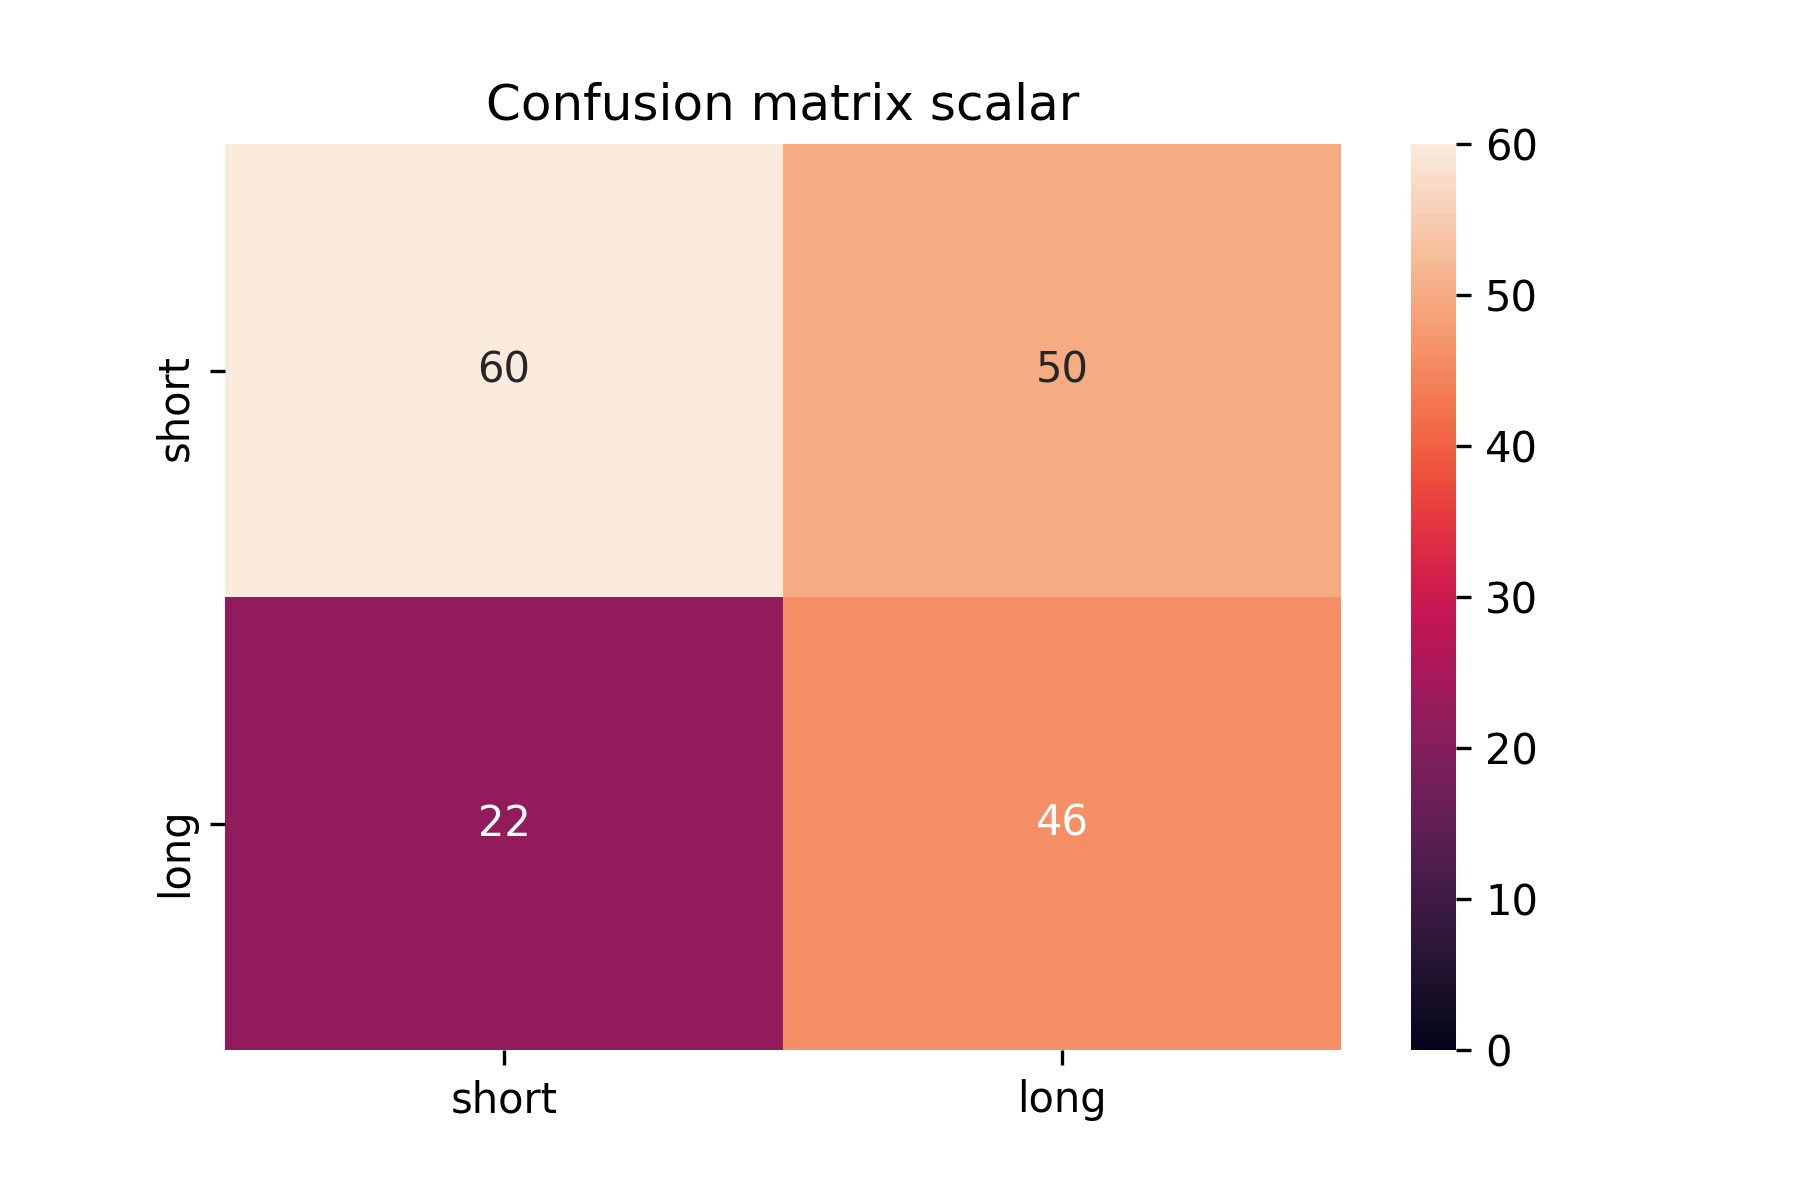
\includegraphics[width=.5\textwidth]{images/results/survival_scalar}

  \caption[Confusion matrix for survival classification]{
    Confusion matrix for survival classification between long survivors and short 
    survivors when using the results from \autoref{sec:scalar-only} that only uses
    radiomic scalar features. Final accuracy is 60\% (106 / 178).
    \label{fig:survival-confusion}
  }
\end{figure}

Since these results are not quite satisfying, future work will be to improve this step.
To do so, the next idea is to use the extracted features from the sister network output,
instead of the siamese network output, and then train a \gls{CPH} model using these features.

This way the siamese network is used to convert the regression problem into a classification 
problem and train a model with it. Then by extracting the hidden features the model can be
converted again into a regression model, already trained.

\ssecc{Write documentation}

Since this project creates a software, some documentation for the software must be written.
Moreover documenting the code is important to allow more people to work on the project.
The project's documentation can be found at \url{https://jmigual.github.io/CNNSurv/}.

This task has taken one week to complete, although some work has already been done while 
writing the code to make the task easier.



\cleardoublepage
% !TEX root = main.tex

\phantomsection
\addcontentsline{toc}{\seccn}{\numberline{}Notation}
\secc*{Notation}
\markboth{NOTATION}{NOTATION}

Through the thesis the following notation will be used:

\begin{table}[H]
  \centering
  \begin{tabular}{l|c|p{6cm}}
     & \textbf{Symbol} & \textbf{Description} \\
    \hhline{===}
    Scalars & \( x \) & \\
    Vectors & \( \bm{x} \) & \\
    Elements of vector & \( \bm{x}_i \) & \( i \)-th element of vector \( \bm{x} \) \\
    Matrices & \(\bm{X}\) & \\
    Desired values & \( \bar{x} \) & Desired value for \( x \) \\
    Predicted values & \( \hat{x} \) & Predicted value for \( x \) \\
    L2-norm & \( ||\bm{x}||_2 \) & \\
    \hline
    NN Layer & \( l \) & \\
    Number of layers & \( L \) & \\
    Units for layer & \( n^{[l]} \) & Units for layer \( l \) \\
    Weights & \( w_{ij}^{[l]} \) & Weight between unit \( i \) of layer \( l \) and unit
    \( j \) of layer \( l - 1 \) \\
    Weight matrix & \( \bm{W}^{[l]} \) & Weight 
    matrix between layers \( l \) and \( l - 1 \), 
    \( \bm{W}^{[l]} \in \mathbb{R}^{n^{[l]} \times n^{[l - 1]}} \). \\
    Activation & \( a_i^{[l]} \) & Activation of unit \( i \) for layer \( l \) \\
    Batch size & \( N \) & \\
  \end{tabular}
  \caption{Thesis' notation}
\end{table}



\cleardoublepage
\printglossaries

\emergencystretch=1em
% \addphantomsec{References}{\seccn}
\printbibliography[heading=bibintocindent, title={References}]{}

\end{document}